\begin{figure*}
	\centering
	\begin{adjustbox}{width=\textwidth}
		\begin{tikzpicture}[auto]
			\tikzstyle{diff} = [draw, circle, scale=0.5]
			\foreach \Sigma in {0,...,5} {
					\node[yshift=-350+\Sigma*30, yslant=0.5, xslant=-1.5, scale=1] (bertrand-blur-\Sigma-1) {
						\includegraphics[width=.15\textwidth]{figures/registration/sift/bertrand_sigma_\Sigma.png}
					};
				}
			\foreach \Sigma in {0,...,5} {
					\node[yshift=-160+\Sigma*20, xshift=30, yslant=0.5, xslant=-1.5, scale=0.5] (bertrand-blur-\Sigma-2) {
						\includegraphics[width=.15\textwidth]{figures/registration/sift/bertrand_sigma_\Sigma.png}
					};
				}
			\foreach \Sigma in {0,...,5} {
					\node[yshift=-50+\Sigma*20, yslant=0.5, xshift=30, xslant=-1.5, scale=0.25] (bertrand-blur-\Sigma-3) {
						\includegraphics[width=.15\textwidth]{figures/registration/sift/bertrand_sigma_\Sigma.png}
					};
				}

			\foreach \Sigma in {1,...,5} {
			\begin{scope}[
					yshift=-365+\Sigma*30, xshift=280,every node/.append style={
							yslant=0.5, xslant=-1.5},yslant=0.5, xslant=-1.5
				]
				\node[] (bertrand-dog-\Sigma-1) {
					\includegraphics[width=.15\textwidth]{figures/registration/sift/dog_bertrand_sigma_\Sigma.png}
				};
				\ifnum \Sigma>2
					\foreach \x in {-.8,-.6,-.4}  {
							\foreach \y in {-.8,-.6,-.4} {
									\fill[red!50] (\x,\y) rectangle (\x+.2,\y+.2);
								}
						}
				\fi;

			\end{scope}
			\ifnum \Sigma>2 {
				\draw[yshift=-365+\Sigma*30, step=2mm, xshift=280, black, yslant=0.5, xslant=-1.5] (-1,-1) grid (0,0);
				\draw[yshift=-365+\Sigma*30, xshift=280, black, yslant=0.5, xslant=-1.5] (-1,-1) rectangle (0,0);

				}
			\fi;
			\ifnum \Sigma=4
				\fill[green, yshift=-365+\Sigma*30, xshift=280, yslant=0.5, xslant=-1.5] (-.6,-.6) rectangle (-.4,-.4)
			\fi;
			}
			\foreach \Sigma in {1,...,5} {
					\node[yshift=-365+\Sigma*30, xshift=140, diff] (diff-\Sigma-1){\Large$-$};
				}



			\foreach \Sigma in {1,...,5} {
					\node[yshift=-170+\Sigma*20, xshift=250, yslant=0.5, xslant=-1.5, scale=0.5] (bertrand-dog-\Sigma-2) {
						\includegraphics[width=.15\textwidth]{figures/registration/sift/dog_bertrand_sigma_\Sigma.png}
					};
				}
			\foreach \Sigma in {1,...,5} {
					\node[yshift=-170+\Sigma*20, xshift=140, diff] (diff-\Sigma-2){\Large$-$};
				}



			\foreach \Sigma in {1,...,5} {
					\node[yshift=-45+\Sigma*20, xshift=250, yslant=0.5, xslant=-1.5, scale=0.25] (bertrand-dog-\Sigma-3) {
						\includegraphics[width=.15\textwidth]{figures/registration/sift/dog_bertrand_sigma_\Sigma.png}
					};
				}
			\foreach \Sigma in {1,...,5} {
					\node[yshift=-45+\Sigma*20, xshift=140, diff] (diff-\Sigma-3){\Large$-$};
				}
			%		($(diff-\Sigma-\x) + (0,5mm)$)
			% draw annotations
			\foreach \x in {1,2,3} {
					\foreach \Sigma in {1,...,5} {
							\draw[-] (bertrand-blur-\Sigma-\x) edge (diff-\Sigma-\x);
						}
					\foreach \Sigma in {0,...,4} {
							\pgfmathtruncatemacro{\nodelabel}{1+\Sigma}
							\draw[-] (bertrand-blur-\Sigma-\x) edge (diff-\nodelabel-\x);
						}
					\foreach \Sigma in {1,...,5} {
							\draw[->] (diff-\Sigma-\x) edge (bertrand-dog-\Sigma-\x);
						}
				}
			\coordinate (a) at (-.5, -.5);
			\node (keypoint) [right] at (10,-6) {Candidate Keypoint (not to scale)};
			\tikzstyle{trans} = [thick,->,>=stealth]
			\path[trans] ([] bertrand-blur-3-2.north west) edge[bend left, out=120, in=90] node[above, sloped] {Down-sample 2x} ([] bertrand-blur-0-3.north west);
			\path[trans] ([xshift=2mm] bertrand-blur-3-1.north west) edge[bend left, out=120, in=90] node[above, sloped] {Down-sample 2x} ([] bertrand-blur-0-2.north west);

			\path[trans] ([] keypoint) edge[] node[] {} ([yshift=-365+4*30, xshift=280, yslant=0.5, xslant=-1.5] a);
			\foreach \x in {0,...,4} {
					\pgfmathtruncatemacro{\nodelabel}{\x+1}
					\path[trans] ([xshift=-10mm] bertrand-blur-\x-1.north west) edge[bend left] node[above, sloped] {$k^{\nodelabel}\sigma$} ([xshift=-10mm] bertrand-blur-\nodelabel-1.north west);
				}
		\end{tikzpicture}
	\end{adjustbox}
	\caption{The imaging model illustrating the relationship between a scene and final low-resolution images due to noise, motion, blur, and sampling.}
	\label{fig:bertrand}
\end{figure*}
Images obtained from multiple vantage points, or at different times, of the same scene, become distorted with respect to each other.
%
Since in MISR the aim is to exploit new information across multiple LR samples, we need to first rectify these distortions and reconcile the images.
%
Effectively this means finding one or more pixel transformations that enable mapping all LR images to a common pixel grid.
%
When the transformations cannot be deduced from first principles (e.g., precise knowledge of the relative motion of the scene and the imaging system) they must be estimated from the LR images.
%
The estimation process can be broken down into three distinct steps: feature detection, feature matching, and mapping function estimation.

\subsection{Feature Detection and Selection}

Feature detection and selection is the process of identifying features of the image that are presumed to be invariant across the multiple images to registered.
%
Note that here by features we mean image artifacts (e.g. edges, contours, line intersections, or corners); in this context encodings or transformations of these image artifacts are called \textit{descriptors}.
%
The CPs are the data that will be used to estimate the transformation \(f\).
%
Therefore, in order that the estimated transformation is accurate, CPs should be robust to noise and image degradation, sufficiently distributed throughout the image, and readily matched in the matching step.

\subsubsection{Harris Corner Detection}
Bentoutou \etal\cite{bentoutou2005automatic} use a Harris detector\cite{harris1988combined} to find corner points, arguing that corners are robust to noise and stable over multiple images.
%
The Harris detector improves on the Moravec\cite{moravec1980obstacle} detector.
%
The Moravec detector starts from the error function \(E_{x,y}(u,v)\) which computes the sum of the squared differences (SSD) between an \(m \times m\) weighted window around a pixel \(X(x, y)\) and weighted windows shifted by \(u,v\) pixels:
\begin{multline}
	\quad E_{x,y}(u,v) \coloneqq \\ \sum_{i,j=-m/2}^{m/2} w_{ij}\left[ X(x_i+ u,y_j+v) - X(x_i, y_j)\right]^2
	\label{moravecerrorfunction}
\end{multline}
where \(x_i \coloneqq x + i\) and \(y_j \coloneqq y+j\).
\begin{figure}
	\centering
	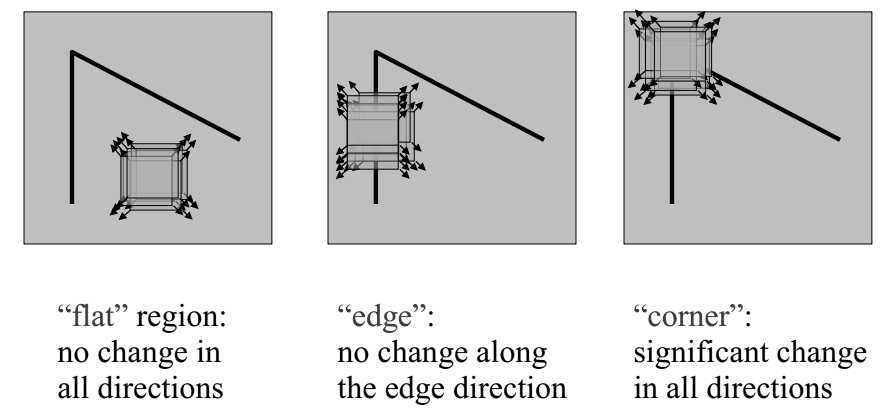
\includegraphics[width=\linewidth,keepaspectratio]{figures/registration/corners.png}
	\caption{Moravec Corner Detector}
	\label{fig:corners}
\end{figure}
Moravec assigns a "corner score" according to the following reasoning (see figure~\ref{fig:corners}):
\begin{framed}
	\begin{enumerate}
		\item If a pixel is in a region of uniform intensity then \(E_{x,y}(u,v)\) is small for all \(u,v\) (since neighboring windows are similar).
		\item If a pixel is on an edge, then \(E_{x,y}(u,v)\) for either \(u > 0\) or \(v > 0\), but not both, is high.
		\item If a pixel is on a corner, then \(E_{x,y}(u,v)\) for \(u > 0\) and \(v > 0\) is high.
	\end{enumerate}
\end{framed}
Therefore the corner score at pixel coordinate \((x,y)\) is \(\min_{u,v} E_{x,y}(u,v)\) in order to select for the third case.
%
Moravec comments that this corner score is not isotropic, i.e. if edges aren't aligned with either the pixel axes or diagonals then \(E_{x,y}(u,v)\) will incorrectly be low.
%
Harris' insight was to linearize \(E_{x,y}(u,v)\) in order to compute a quantity more closely related to the intensity variation in a local
neighborhood of a pixel:
\begin{equation}
	X(x_i + u,y_j + v) \approx  X(x_i,y_j) + \frac{\partial X}{\partial u}u + \frac{\partial X }{\partial v} v
\end{equation}
where the partial derivatives are taken at \((x,y)\).
%
This implies
\begin{align}
	E_{x,y}(u,v) & \approx \sum_{i,j=-m/2}^{m/2} w_{ij} \left[ X_u u + X_v v\right]^2                 \\
	             & = \sum_{i,j=-m/2}^{m/2} w_{ij} \left[ X_u^2 u^2 + X_v^2 v^2 + 2 X_u X_v u v\right] \\
	             & = \left[ u,v \right] \begin{bmatrix}
		\sum w_{ij}X_u^2   & \sum w_{ij}X_u X_v \\
		\sum w_{ij}X_u X_v & \sum w_{ij}X_v^2   \\
	\end{bmatrix}  \begin{bmatrix}
		u \\
		v
	\end{bmatrix}          \\
	             & = \left[ u,v \right] M  \begin{bmatrix}
		u \\
		v
	\end{bmatrix} \label{eqn:structurematrix}
\end{align}
where \(X_u \coloneqq \partial X/\partial u\) and similarly \(X_v\).
%
The matrix in eqn.~\eqref{eqn:structurematrix}, called the \textit{structor tensor} or \textit{second-moment matrix} \(M\), is the quantity Harris investigated.
%
Harris reasoned that the cases of Moravec correspond to conditions on the eigenvalues \(\lambda_1, \lambda_2\) of \(M\):
\begin{framed}
	\begin{enumerate}
		\item If \(\lambda_1 \approx \lambda_2 \approx 0\) then \(X(x,y)\) is in a region of uniform intensity.
		\item If \(\lambda_1 \gg \lambda_2\) or \(\lambda_2 \gg \lambda_1\) then \(X(x,y)\) is on an edge.
		\item \(\lambda_1 \approx \lambda_2 > 0\) then \(X(x,y)\) is on a corner.
	\end{enumerate}
\end{framed}
Notice that if \(w_{ij} = 1\) then this is just the gradient covariance of the image and the Harris detector is essentially a local Principle Components Analysis (PCA).
%
In fact Harris doesn't actually compute the eigenvalues but instead a related quantity called the ``strength'':
\begin{align}
	S & \coloneqq \lambda_1 \lambda_2 - \kappa (\lambda_1 + \lambda_2)^2 \\
	  & = \det(M) - \kappa \operatorname{trace}^2(M)
	\label{eqn:strength}
\end{align}
%
Hence Bentoutou \etal~first compute a gradient map of the image using a first order Gaussian derivative filter.
%
They then threshold\anote{threshold} the gradient map at the average gradient value, thereby extracting only sufficiently "interesting" regions, and compute the strength \(S\) for all pixels.
%
They also apply Non-maximum Suppression\anote{nms} (NMS) using a \(3 \times 3\) window and further threshold the remaining non-zero strength values at a threshold of 1\% of maximum observed strength.
%
Finally only the ``strongest'' \(n\) corners are kept.

\subsubsection{SIFT}\label{sec:sift}

\begin{figure}
	\centering
	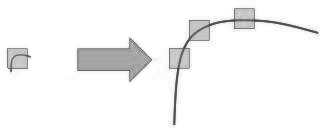
\includegraphics[width=\linewidth,keepaspectratio]{figures/registration/sift/sift_scale_invariant.png}
	\caption{Harris Detector failing to recognize the right image as a corner.}
	\label{fig:sift_harris}
\end{figure}
One issue with Harris detectors is that they're not invariant to scale (see figure~\ref{fig:sift_harris}).
%
Zahra \etal\cite{zahrasift} resolves this issue by using the Scale Invariant Feature Transform\cite{lowe2004distinctive} (SIFT) to identify CPs that, as the name implies, are invariant across multiple scales.
%
SIFT identifies scale invariant and noise robust features of an image, called \textit{keypoints}, by first finding candidate points with high local curvature at multiple scales and then culling according to some heuristics.
\begin{figure*}
	\pgfplotstableread[]{figures/registration/sift/subgrad_hists.csv}\subgradhists;
	\tikzstyle{every picture}+=[remember picture]
	\tikzset{
		pics/greensquare/.style args={#1/#2/#3}{
				code = {
						\draw[green, line width=.5mm] (#1,#2) rectangle (#1+#3, #2+#3);
					}
			},
		subgradbin/.pic={
				\foreach \i in {0.0, 1.0} {
						\pgfmathsetmacro{\x}{0.5+\i*2*.08825};
						\foreach \j in {0.0, 1.0} {
								\pgfmathsetmacro{\y}{0.5+\j*2*.08825};
								\pic[] {greensquare=\x/\y/2*.08825};
							};
					};
			},
		pics/subgradbins/.style args={#1}{
				code = {
						\foreach \x in {0,1,2,3} {
								\pgfmathtruncatemacro{\angle}{#1+\x*90}
								\pic[rotate around={\angle:(0.5,0.5)}] {subgradbin};
							}
					}
			},
		pics/edgehistogram/.style args={#1/#2}{
				code={
						\begin{axis}[area style, width=2.5cm,height=2.5cm, hide axis, at={(#1cm,#2cm)}]
							\addplot+[ybar interval] plot coordinates {
									(-0.50, 2) (0.5, 4) (1.5, 5) (2.5, 3) (3.5, 2) (4.5, 2) (5.5, 0)
								};
							\path
							\foreach[count=\i from 0] \v in {2, 4, 5, 3, 2, 2} {
									(\i, \v) node[below] {\tiny\v}
								};
						\end{axis}
					}
			},
		pics/randomedgehistogram/.style args={#1/#2}{
				code={
						\node (hist-#1#2) at (#1cm+.5cm,#2cm+.5cm) {};% {#1,#2};
						\begin{axis}[area style, width=2.5cm,height=2.5cm, hide axis, at={(#1cm,#2cm)}]
							\pgfmathtruncatemacro{\rowindex}{#1*4+#2}
							\pgfplotstablegetelem{\rowindex}{[index]0}\of{\subgradhists}\pgfmathtruncatemacro{\na}{\pgfplotsretval};
							\pgfplotstablegetelem{\rowindex}{[index]1}\of{\subgradhists}\pgfmathtruncatemacro{\nb}{\pgfplotsretval};
							\pgfplotstablegetelem{\rowindex}{[index]2}\of{\subgradhists}\pgfmathtruncatemacro{\nc}{\pgfplotsretval};
							\pgfplotstablegetelem{\rowindex}{[index]3}\of{\subgradhists}\pgfmathtruncatemacro{\nd}{\pgfplotsretval};
							\pgfplotstablegetelem{\rowindex}{[index]4}\of{\subgradhists}\pgfmathtruncatemacro{\ne}{\pgfplotsretval};
							\pgfplotstablegetelem{\rowindex}{[index]5}\of{\subgradhists}\pgfmathtruncatemacro{\nf}{\pgfplotsretval};
							\pgfplotstablegetelem{\rowindex}{[index]6}\of{\subgradhists}\pgfmathtruncatemacro{\ng}{\pgfplotsretval};
							\pgfplotstablegetelem{\rowindex}{[index]7}\of{\subgradhists}\pgfmathtruncatemacro{\nh}{\pgfplotsretval};
							\addplot+[ybar interval] plot coordinates {
									(-0.50, \na)
									(0.5, \nb)
									(1.5, \nc)
									(2.5, \nd)
									(3.5, \ne)
									(4.5, \nf)
									(5.5, \ng)
									(6.5, \nh)
									(7.5, 0)
								};
							\draw
							\foreach[count=\i from 0] \v in {\na, \nb, \nc, \nd, \ne, \nf, \ng, \nh} {
									(\i, \v) node[below] {\scalebox{.3}{\v}}
								};
						\end{axis}
					}
			},
		array/.style={
				draw,
				minimum width=2em,
				minimum height=2em,
				outer sep=0pt
			},
	}
	\newcommand*{\siftwidth}{.5\linewidth}
	\newcommand*{\length}{sqrt((2.*x^2+2.*y^2)^2 + (8.*x^2*y^2)^2 )}
	\pgfplotsset{
		dominantorientationaxis/.style={
				enlargelimits = false,
				view={0}{90},
				xmin=0, xmax=1, ymin=0, ymax=1,
				ytick distance=1/16,
				xtick distance=1/16,
				axis equal image, grid=both,
				minor grid style={black},
				major grid style={black},
				axis equal image,
			},
	}
	\pgfplotsset{ticks=none}
	\begin{subfigure}{\siftwidth}
		\centering
		\begin{tikzpicture}
			\begin{axis}[dominantorientationaxis]
				\addplot[on layer=axis background] graphics[xmin=0, xmax=1, ymin=0, ymax=1]
					{figures/registration/sift/bert_keypoint.png};
				\addplot[redarrow,quiver={u=\thisrow{u},v=\thisrow{v}}] table {figures/registration/sift/grads.csv};
				\node[dot=5pt](keypoint) at (0.5,0.5) {};
			\end{axis}
			\node (keyp) at (4,6.5) {Keypoint};
			\draw[redarrow] (keyp)--(keypoint);
		\end{tikzpicture}
		\caption{Keypoint neighborhood.} \label{fig:siftdescriptora}
	\end{subfigure}
	\pgfmathsetmacro{\rot}{54}
	\pgfmathsetmacro{\br}{sqrt(2)*.5/2}
	\begin{subfigure}{\siftwidth}
		\centering
		\begin{tikzpicture}
			\begin{axis}[dominantorientationaxis, set layers]
				\addplot[on layer=axis background] graphics[xmin=0, xmax=1, ymin=0, ymax=1]
					{figures/registration/sift/bert_keypoint.png};
				\addplot[redarrow,quiver={u=\thisrow{u},v=\thisrow{v}}] table {figures/registration/sift/grads.csv};
				\node[dot=5pt](keypoint) at (0.5,0.5) {};

				\draw[yellow] (0.5, 0.5) circle [radius=.5];
				\pic[rotate around={\rot:(0.5,0.5)}] {greensquare=.1464/.1464/.707};
				\draw[line width=2pt,red,-latex](.5,.5)--(.5+0.3579, 1);
				\coordinate (gausscircle) at (.75,.25);
				\coordinate (dominantgrad) at (.5+0.25,.5+.35);
				\coordinate (gradsquare) at (.5-\br,.5+\br);
			\end{axis}
			\node (gausswin) at (5,-0.5) {Gradient Window};
			\node (gradwin) at (1,6.5) {Gaussian Window};
			\node (domin) at (4,6.5) {Majority Gradient};
			\draw[redarrow] (gausswin)--(gausscircle);
			\draw[redarrow] (gradwin)--(gradsquare);
			\draw[redarrow] (domin)--(dominantgrad);
		\end{tikzpicture}
		\caption{Oriented and filterd keypoint gradient neigbhorhood.} \label{fig:siftdescriptorb}
	\end{subfigure}
	\vskip\baselineskip
	\begin{subfigure}{\siftwidth}
		\centering
		\begin{tikzpicture}
			\begin{scope}[rotate=\rot,transform shape,local bounding box=scope1]
				\clip[](1.95,1.99) rectangle (6.0,6.03);
				\begin{axis}[dominantorientationaxis, rotate around={-\rot:(.5,.5)}, grid=none]
					\addplot[on layer=axis background] graphics[xmin=0, xmax=1, ymin=0, ymax=1]
						{figures/registration/sift/bert_keypoint.png};
					\addplot[redarrow,quiver={u=\thisrow{u},v=\thisrow{v}}] table {figures/registration/sift/grads.csv};
					\pic[] {subgradbins=\rot};
					\node[dot=5pt](keypoint) at (0.5,0.5) {};
				\end{axis}
			\end{scope}
			\begin{scope}[shift={($(scope1.south)-(0,1cm)$)}]
				\coordinate (gradbin) at (0.5,5.5);
				\node (gradb) at (2,6.5) {Gradient bin};
				\draw[redarrow] (gradb)--(gradbin);
			\end{scope}
		\end{tikzpicture}
		\caption{16 Keypoint neigbhorhood gradient bins.} \label{fig:siftdescriptorc}
	\end{subfigure}
	\begin{subfigure}{\siftwidth}
		\centering
		\begin{tikzpicture}
			\begin{scope}[rotate=\rot,transform shape,local bounding box=scope1]
				\foreach \i [evaluate=\i as \x using \i*1.0] in {0,...,3}{
						\foreach \j [evaluate=\j as \x using \j*1.0] in {0,...,3}{
								\pic {greensquare=\i/\j/1.0};
								\pic {randomedgehistogram=\i/\j};
							}
					}
				\node[dot=5pt](keypoint) at (2.0,2.0) {};
			\end{scope}
			\node (histb) at (2,5.5) {Histogram of gradient orientations};
			\draw[redarrow] (histb)--(hist-32);
			\begin{scope}[shift={($(scope1.south)-(0,1cm)$)}]
				\matrix (A) [matrix of math nodes, nodes={array, anchor=center}, column sep=-\pgflinewidth] {
					\pgfmathtruncatemacro{\rowindex}{3}
					\pgfplotstablegetelem{\rowindex}{[index]0}\of{\subgradhists}\pgfmathprintnumber[fixed,precision=0]{\pgfplotsretval},
					\pgfplotstablegetelem{\rowindex}{[index]1}\of{\subgradhists}\pgfmathprintnumber[fixed,precision=0]{\pgfplotsretval},
					\pgfplotstablegetelem{\rowindex}{[index]2}\of{\subgradhists}\pgfmathprintnumber[fixed,precision=0]{\pgfplotsretval},
					\pgfplotstablegetelem{\rowindex}{[index]3}\of{\subgradhists}\pgfmathprintnumber[fixed,precision=0]{\pgfplotsretval},
					\pgfplotstablegetelem{\rowindex}{[index]4}\of{\subgradhists}\pgfmathprintnumber[fixed,precision=0]{\pgfplotsretval},
					\pgfplotstablegetelem{\rowindex}{[index]5}\of{\subgradhists}\pgfmathprintnumber[fixed,precision=0]{\pgfplotsretval},
					\pgfplotstablegetelem{\rowindex}{[index]6}\of{\subgradhists}\pgfmathprintnumber[fixed,precision=0]{\pgfplotsretval},
					\pgfplotstablegetelem{\rowindex}{[index]7}\of{\subgradhists}\pgfmathprintnumber[fixed,precision=0]{\pgfplotsretval} &
					\pgfmathtruncatemacro{\rowindex}{2}
					\pgfplotstablegetelem{\rowindex}{[index]0}\of{\subgradhists}\pgfmathprintnumber[fixed,precision=0]{\pgfplotsretval},
					\pgfplotstablegetelem{\rowindex}{[index]1}\of{\subgradhists}\pgfmathprintnumber[fixed,precision=0]{\pgfplotsretval},
					\pgfplotstablegetelem{\rowindex}{[index]2}\of{\subgradhists}\pgfmathprintnumber[fixed,precision=0]{\pgfplotsretval},
					\pgfplotstablegetelem{\rowindex}{[index]3}\of{\subgradhists}\pgfmathprintnumber[fixed,precision=0]{\pgfplotsretval},
					\pgfplotstablegetelem{\rowindex}{[index]4}\of{\subgradhists}\pgfmathprintnumber[fixed,precision=0]{\pgfplotsretval},
					\pgfplotstablegetelem{\rowindex}{[index]5}\of{\subgradhists}\pgfmathprintnumber[fixed,precision=0]{\pgfplotsretval},
					\pgfplotstablegetelem{\rowindex}{[index]6}\of{\subgradhists}\pgfmathprintnumber[fixed,precision=0]{\pgfplotsretval},
					\pgfplotstablegetelem{\rowindex}{[index]7}\of{\subgradhists}\pgfmathprintnumber[fixed,precision=0]{\pgfplotsretval} &
					\cdots\cdots\cdots                                                  &
					\pgfmathtruncatemacro{\rowindex}{12}
					\pgfplotstablegetelem{\rowindex}{[index]0}\of{\subgradhists}\pgfmathprintnumber[fixed,precision=0]{\pgfplotsretval},
					\pgfplotstablegetelem{\rowindex}{[index]1}\of{\subgradhists}\pgfmathprintnumber[fixed,precision=0]{\pgfplotsretval},
					\pgfplotstablegetelem{\rowindex}{[index]2}\of{\subgradhists}\pgfmathprintnumber[fixed,precision=0]{\pgfplotsretval},
					\pgfplotstablegetelem{\rowindex}{[index]3}\of{\subgradhists}\pgfmathprintnumber[fixed,precision=0]{\pgfplotsretval},
					\pgfplotstablegetelem{\rowindex}{[index]4}\of{\subgradhists}\pgfmathprintnumber[fixed,precision=0]{\pgfplotsretval},
					\pgfplotstablegetelem{\rowindex}{[index]5}\of{\subgradhists}\pgfmathprintnumber[fixed,precision=0]{\pgfplotsretval},
					\pgfplotstablegetelem{\rowindex}{[index]6}\of{\subgradhists}\pgfmathprintnumber[fixed,precision=0]{\pgfplotsretval},
					\pgfplotstablegetelem{\rowindex}{[index]7}\of{\subgradhists}\pgfmathprintnumber[fixed,precision=0]{\pgfplotsretval}
					\\};
				\draw[decorate,decoration={brace, amplitude=10pt, raise=5pt, mirror}]
				(A-1-1.south west) to node[black,midway,below= 15pt] {$16 \times 8 = 128$ entries} (A-1-4.south east);%
				\draw[redarrow] (hist-03) -- (A-1-1);
				\draw[redarrow] (hist-02) -- (A-1-2);
				\draw[redarrow] (hist-01) -- (A-1-3);
				\draw[redarrow] (hist-00) -- (A-1-3);
				\foreach \i in {1,...,2}{
						\foreach \j in {0,...,3}{
								\draw[redarrow] (hist-\i\j) -- (A-1-3);
							}
					}
				\draw[redarrow] (hist-33) -- (A-1-3);
				\draw[redarrow] (hist-31) -- (A-1-3);
				\draw[redarrow] (hist-32) -- (A-1-3);
				\draw[redarrow] (hist-30) -- (A-1-4);
			\end{scope}
		\end{tikzpicture}
		\caption{Histogram of gradient orientations descriptor.} \label{fig:siftdescriptord}
	\end{subfigure}
	\caption{Sift keypoint descriptor construction.} \label{fig:siftdescriptor}
\end{figure*}


%
It then "describes" these keypoints by a rotation invariant and noise robust representation.
%
The algorithm consists of five steps:
%
\begin{framed}
	\begin{enumerate}
		\item Scale-space pyramid construction: a sequence of increasingly sub-sampled and more strongly Gaussian filtered images is computed. The sequence of differences of these images is also computed; the sequence of differenced images approximates the multi-scale Laplacian of Gaussians\anote{log} (LoG) of the image (see figure~\ref{fig:siftpyramid}).
		\item Keypoint detection: candidate keypoints are points on edges with curvature, i.e. extrema along scale and space dimensions in the LoG pyramid (see figure~\ref{fig:siftpyramid}).
		\item Keypoint selection: candidate keypoints are more precisely localized using an iterative process. Keypoints of low-contrast (therefore sensitive to noise) or on edges of low curvature\anote{smallcurvature} are culled.
		\item Keypoint orientation assignment: orientation is assigned to each keypoint by taking a weighted majority vote of all gradient orientations in a neighborhood of the keypoint (see figure~\ref{fig:siftdescriptorb}). Large minority votes (80\% of majority) are used to create more keypoints at the same pixel point.
		\item Keypoint descriptor computation: for each keypoint the descriptor is computed by partitioning the keypoint's neighborhood into \(2^k\) sub-neighborhoods, computing an 8-bin histogram of oriented gradients\anote{hog} (HOG) in each sub-neighborhood, and concatenating (see figure~\ref{fig:siftdescriptord}). In Lowe \etal\cite{lowe2004distinctive} \(2^4=16\) sub-neighborhoods are used to produce an \(8\times16 = 128\) entry length descriptor. The descriptor is also normalized to unit length in order to make it invariant to luminance (intensity).
	\end{enumerate}
\end{framed}

SIFT is indeed effective as a CP detector but unfortunately it is patented.
%
Alternatives include Binary Robust Invariant Scalable Keypoints\cite{leutenegger2011brisk}, and Oriented FAST and rotated BRIEF\cite{rublee2011orb} (which itself consists of applying Features from accelerated segment test\cite{rosten2006machine} to detect points of interest and Binary Robust Independent Elementary Features\cite{calonder2010brief} to compute descriptors).

\subsection{Feature Matching}

After robust features are identified in the reference image and the displaced images, they need to be matched.
%
For example for SIFT, where the descriptors are designed to be invariant across images, Euclidean distance using a \(k\)-d tree\anote{kdtree} can be used to efficiently match keypoint descriptors.
%
Although this often leads to false-positive matches (Zahra \etal~resolve this by using Random Sample Consensus (RANSAC)\anote{ransac}) it's a natural feature matching method.
%
In other cases the matching mechanism is not so straightforward; for a class of algorithms called area-based or intensity-based algorithms, that in fact combine the feature detection and matching step into one, matching involves comparing summaries of patches in the reference image and the displaced image.

\subsubsection{Convex Hull Edges}
%
One technique that matches features explicitly is Point Matching Using Convex Hull Edges\cite{Goshtasby1985}.
%
It operates on the principle that the convex hull\anote{convexhull} of a set of points is invariant under translation, rotation, and scaling.
%
Goshtasby \etal~further argue that a noised set of points will most likely have elements deleted or added in its interior and therefore register the boundaries of the respective convex hulls of the to-be-registered image and the reference image (see figure~\ref{fig:convexhulledges}).
%
\begin{figure}[!htbp]
	\begin{subfigure}{\linewidth}
		\centering
        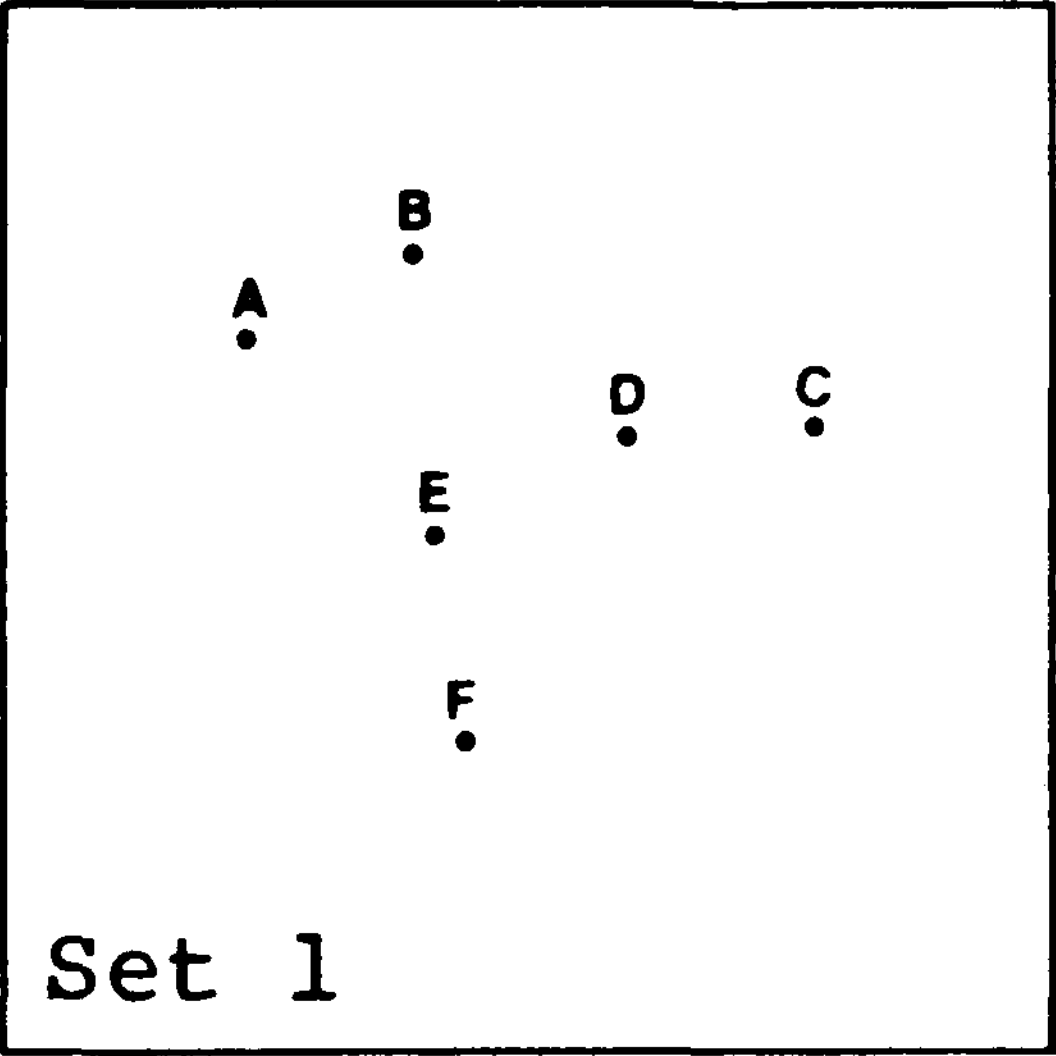
\includegraphics[width=.48\textwidth]{figures/registration/convex/set1.png}
        \raisebox{1px}{
			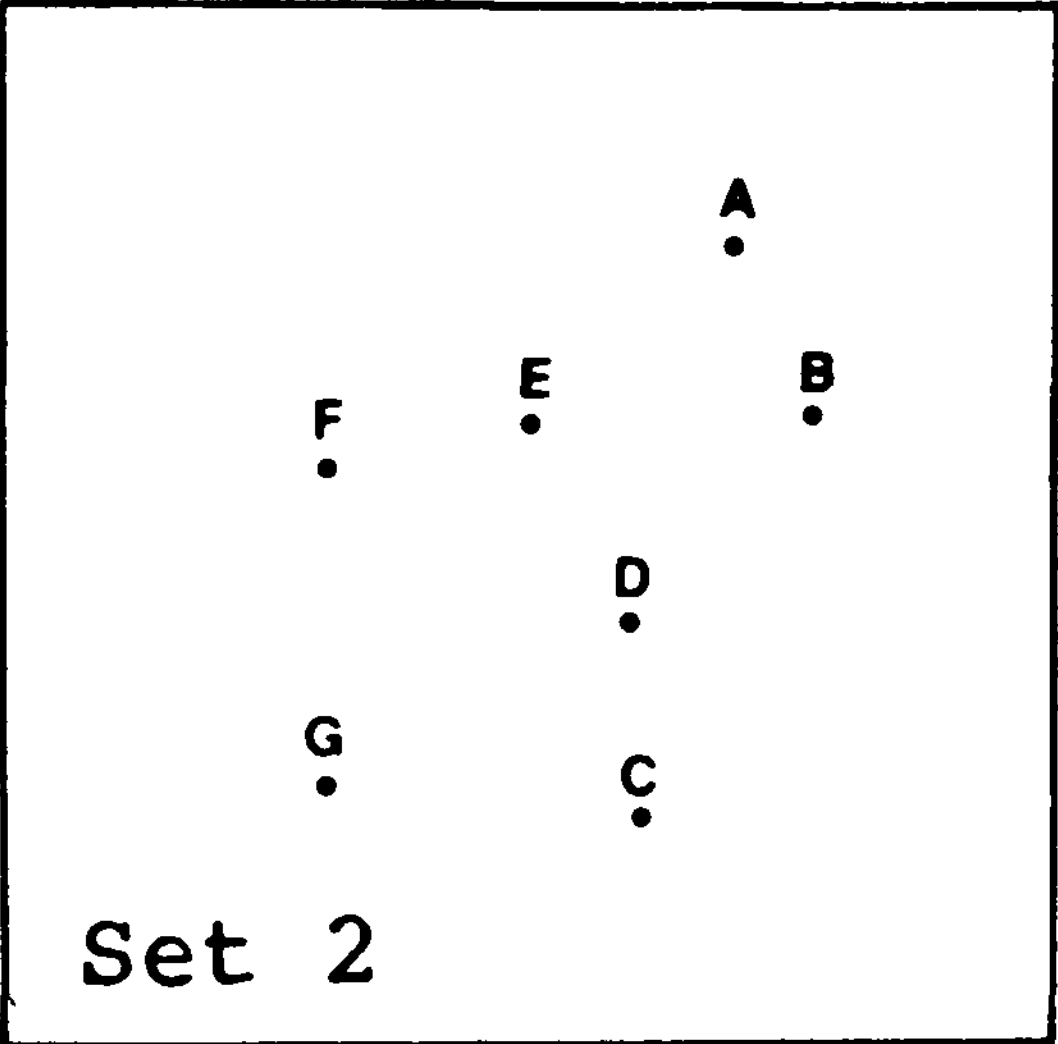
\includegraphics[width=.48\textwidth]{figures/registration/convex/set2.png}
		}
		\caption{Two sets of points. Set 2 is 90 degrees rotated and has extra point \(G\).} \label{fig:twosetsofpoints}
	\end{subfigure}
	\vskip\baselineskip
	\begin{subfigure}{\linewidth}
		\centering
		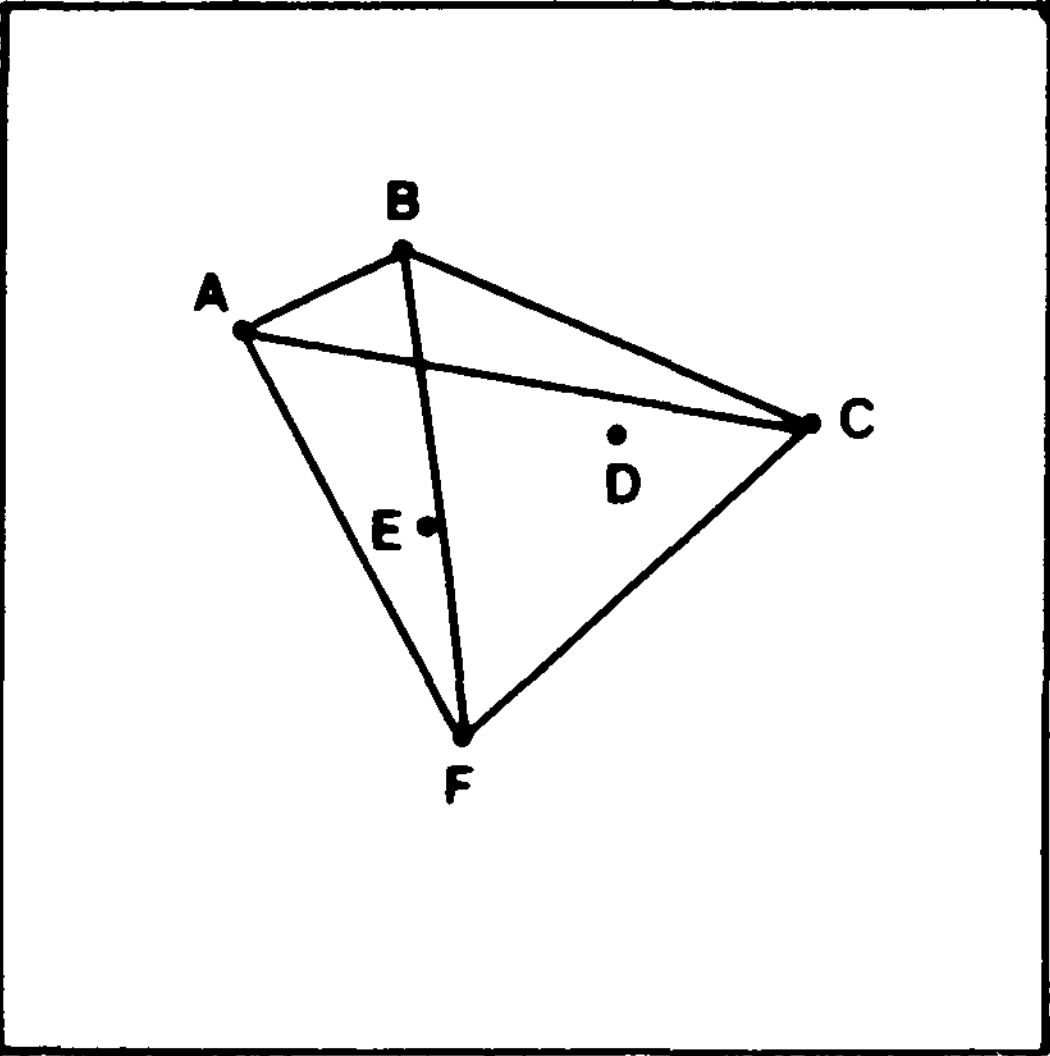
\includegraphics[width=.48\textwidth]{figures/registration/convex/complete_graph_set1.png}
		\raisebox{0.5px}{
			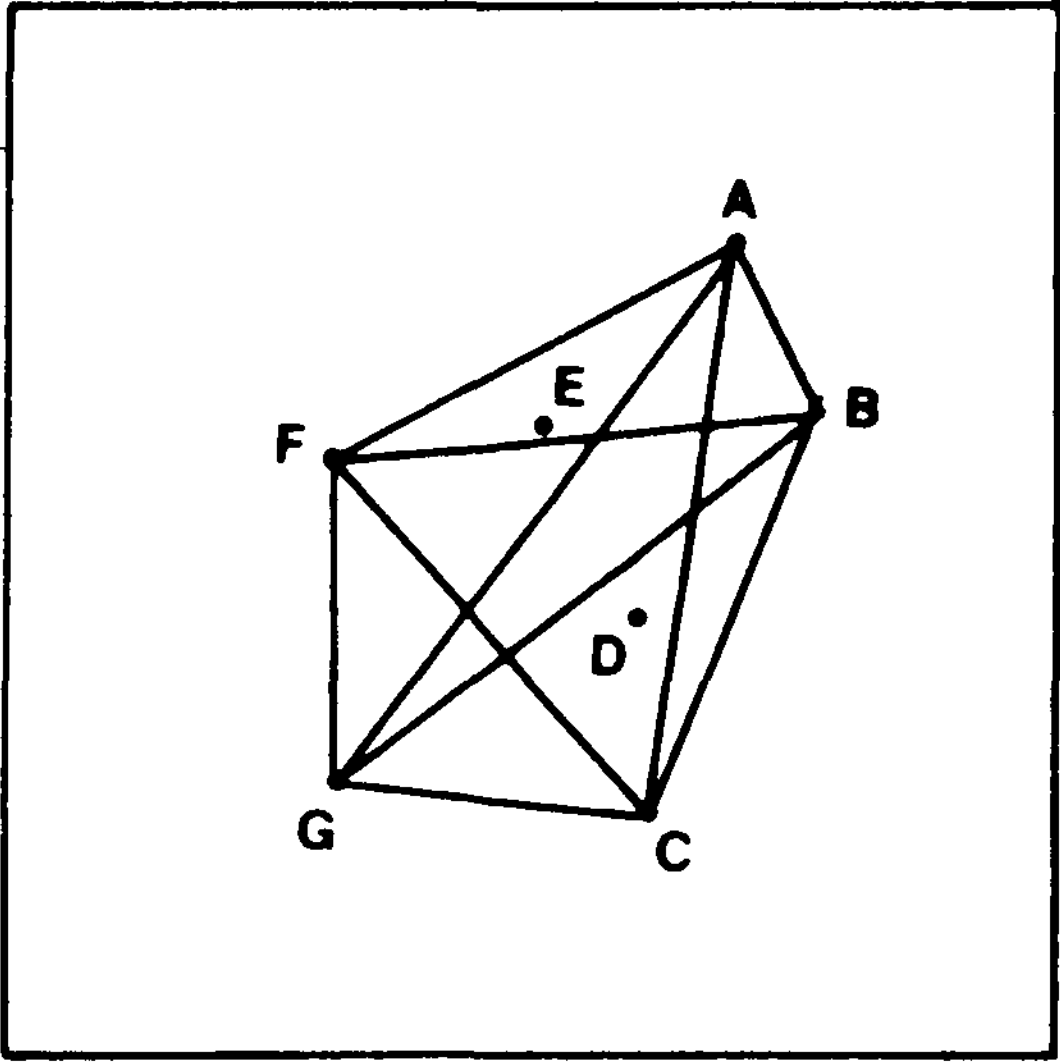
\includegraphics[width=.48\textwidth]{figures/registration/convex/complete_graph_set2.png}
		}
		\caption{Convex hull complete graph edges of two sets, used by the point matching using convex hull edges algorithm.} \label{fig:twoconvexcomplete}
	\end{subfigure}
	\caption{Point matching using convex hull edges \cite{Goshtasby1985}.}
	\label{fig:convexhulledges}
\end{figure}

The key part of the algorithm (after computing the convex hull of the control points) is estimating transformation parameters between convex hull boundaries \(C_1, C_2\):
%
\begin{framed}
	\begin{enumerate}
		\item Determine the complete graphs\anote{completegraph} \(G_1=(V_1, E_1)\), \(G_2 = (V_2,E_2)\) of \(C_1\) and \(C_2\). Then \[|E_1| = \frac{|V_1| (|V_1|-1)}{2}\] (\(|V_1|\) "choose" 2) and similarly \(|E_2|\). Since there are 2 ways to match any undirected edge we extend \(E_2\) to include reverse directed edges and therefore \[|E_2| = |V_2| (|V_2|-1)\]
		\item For each possible pairing of edges \(e_i, e_j\) in \(E_1, E_2\) compute the rotation \(R_{ij}\), scaling \(S_{ij}\), and translation \(T_{ij}\).
		\item Given the composite transformation \(R_{ij} \circ S_{ij} \circ T_{ij}\) count the number \(N_{ij}\) of other points in \(C_1, C_2\) that also match (within a threshold distance \(D\)).
		\item \(N_{IJ} = \max_{i,j} N_{ij}\) and \(R_{IJ}\, \circ S_{IJ}\, \circ\, T_{IJ}\) are the transformation parameters between the control points.
	\end{enumerate}
\end{framed}
%
Note that this procedure operates on one set of control points at a time and that there could be many such matchings computed before final registration between images can be performed.

\subsubsection{Normalized Cross-correlation}
The simplest strategy for matching by region is to grid-search\anote{gridsearch} the space of possible translational shifts \(\Delta x, \Delta y\) and assess the quality of the registration for a given shift using a similarity metric.
%
One such similarity metric is Normalized Cross-correlation (NCC); for two image patches \(X, Y\) (with the same width, height) NCC is defined in a straightforward way
\begin{multline}
	\operatorname{NCC}(X, Y) \coloneqq \\ \frac{\sum_{x,y} \left(X(x,y) - \hat{X}\right) \left(Y(x,y) - \hat{Y}\right)}{\sqrt{\sum_{x,y} \left(X(x,y) - \hat{X}\right)^2} \sqrt{ \sum_{x,y} \left(Y(x,y) - \hat{Y}\right)^2 }}
\end{multline}
where \(\hat{X}, \hat{Y}\) are mean patch values.

\begin{figure}[!htbp]
	\begin{subfigure}{\linewidth}
		\centering
		\begin{adjustbox}{width=.8\textwidth}
			\begin{tikzpicture}
				\node[inner sep=0pt, xshift=50, yshift=-50] (shiftedcat) {
					{\transparent{.5}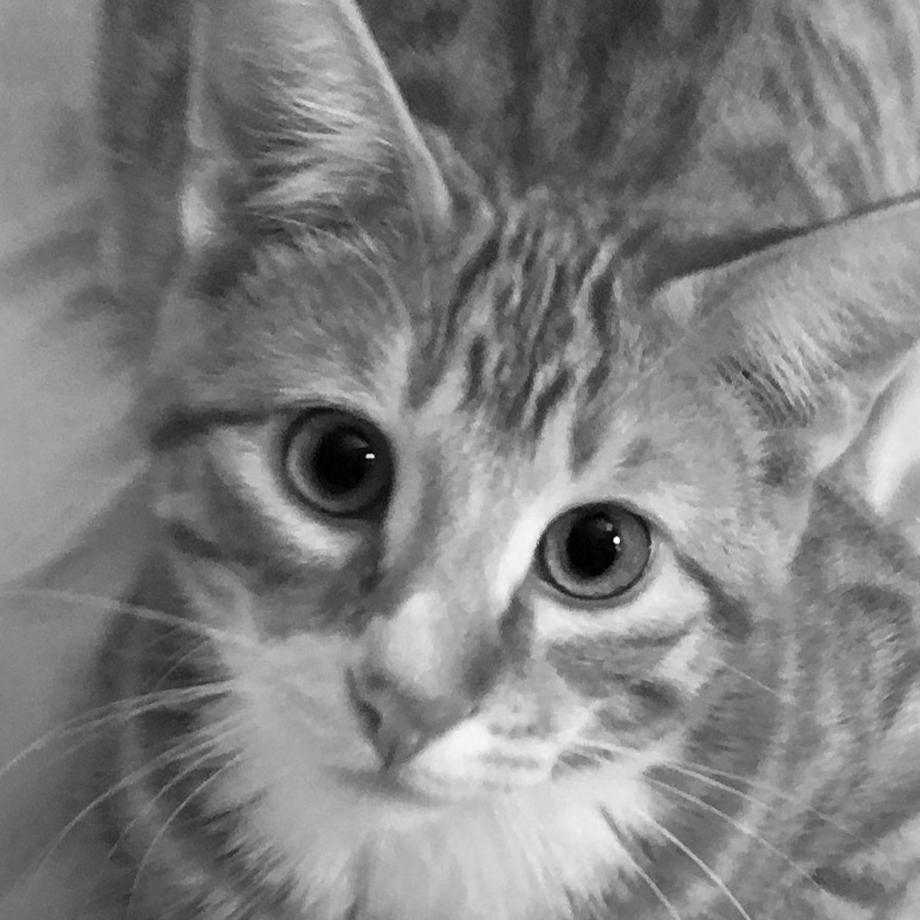
\includegraphics[]
							{figures/registration/cross-correlation/trimmed_cat.jpg}
						}};
				\node[inner sep=0pt, xshift=-50pt, yshift=50pt] (shiftedcat) {
					{\transparent{0.5}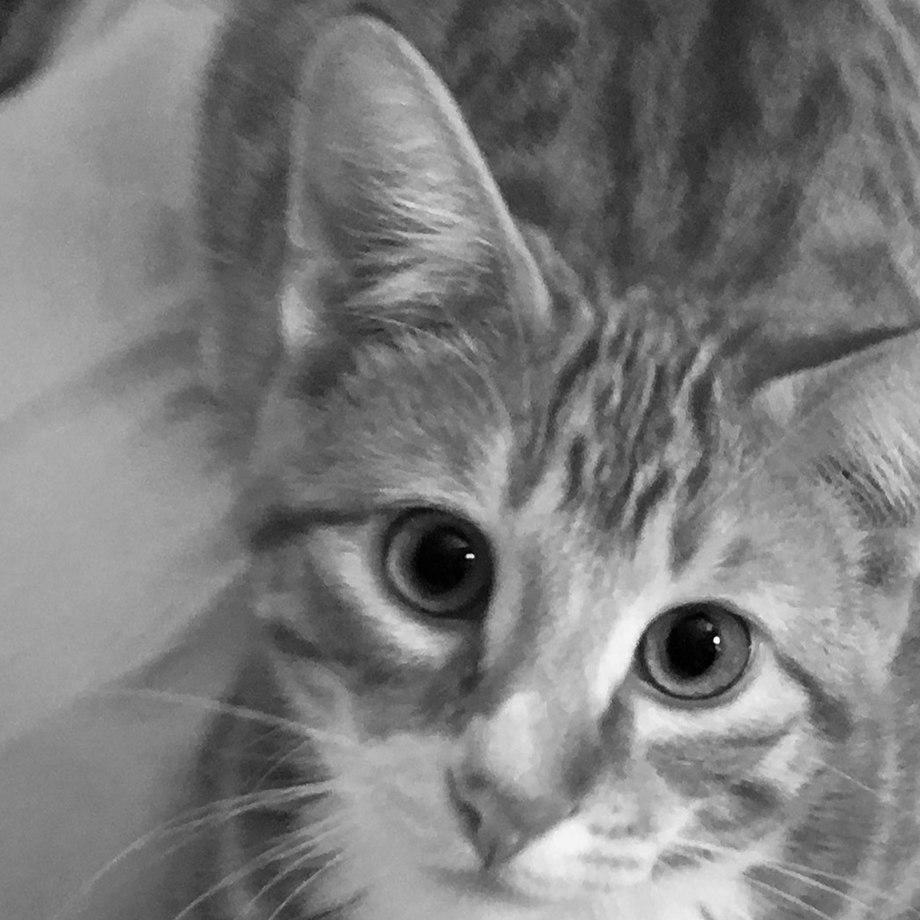
\includegraphics[]
							{figures/registration/cross-correlation/shifted_trimmed_cat.jpg}
						}};
				\draw[red, line width=1mm] (-250pt,-250pt) rectangle (250pt,250pt);
				\node(corrwin) at (0,250pt) {};
				\node[label={[label distance=1cm]:\scalebox{5}{Fixed cross-correlation window}}] (corrw) at (0,600pt) {};
				\draw[redarrow, line width=1mm] (corrw)--(corrwin);
			\end{tikzpicture}
		\end{adjustbox}
		\caption{100 pixel shifted images.} \label{fig:shiftedcat}
	\end{subfigure}
	\vskip\baselineskip
	\begin{subfigure}{\linewidth}
		\centering
		\begin{tikzpicture}
			\begin{axis}
				\addplot3 [surf, mesh/rows=19, mesh/ordering=x varies]
				table[col sep=comma] {figures/registration/cross-correlation/surf.csv};
				\node[above] at (axis cs:-110,-110,224141) {\((-100, -100)\)};
			\end{axis}
		\end{tikzpicture}
		\caption{Cross-correlation for various \(\Delta x, \Delta y\) shifts, with highest correlation at the shift.}
		\label{fig:crosscorr}
	\end{subfigure}
	\vskip\baselineskip
	\begin{subfigure}{\linewidth}
		\centering
		\begin{tikzpicture}
			\begin{axis}
				\addplot3 [surf, mesh/rows=19, mesh/ordering=x varies]
				table[col sep=comma] {figures/registration/cross-correlation/delta_surf.csv};
				\node[above] at (axis cs:-110,-110,1) {\((-100, -100)\)};
			\end{axis}
		\end{tikzpicture}
		\caption{Phase-correlation for various \(\Delta x, \Delta y\) shifts, with single peak at the correct shift.}
		\label{fig:phasecorr}
	\end{subfigure}
	\caption{Cross-correlation feature matching.}
	\label{fig:nccshift}
\end{figure}

%
The NCC image registration technique performs a grid-search over possible shifts and compute the cross-correlation of the shifted images (see figure~\ref{fig:shiftedcat}) (usually over a fixed cross-correlation window rather than the entire image for the sake of computational efficiency).
%
The maximum response as a function \(\Delta x, \Delta y\) is the imputed translation between the images (see figure~\ref{fig:crosscorr}).
%
An alternative but closely related method is \textit{phase correlation}, based on the Fourier shift theorem\anote{fouriershift}  (the value of going to Fourier space is availability of highly optimized algorithms for computing the Fourier transform).
%
Let \(\mathcal{X}(u,v) = \mathcal{F}\{X(x,y)\}, \; \mathcal{Y}(u,v) = \mathcal{F}\{Y(x,y)\}\) be the Fourier transforms of the displaced images.
%
Then
\[
	\mathcal{X} = \mathcal{Y}  e^{-2 \pi i (\frac{u \Delta x}{M} + \frac{v \Delta y}{N})}
\]
where \(N,M\) are the dimensions of the images
%
and the \textit{normalized cross-power spectrum}
\begin{align}
	R(u,v) & \coloneqq \frac{\mathcal{X}\odot \mathcal{Y}^{*}}{|\mathcal{X} ||\mathcal{Y}^{*} |}                                                                                                                    \\
	       & = \frac{\mathcal{X}\odot \mathcal{X}^{*} \, e^{2 \pi i (\frac{u \Delta x}{M} + \frac{v \Delta y}{N})}}{|\mathcal{X} ||\mathcal{X}^{*} \, e^{-2 \pi i (\frac{u \Delta x}{M} + \frac{v \Delta y}{N})} |} \\
	       & = \frac{\mathcal{X}\odot \mathcal{X}^{*} \, e^{2 \pi i (\frac{u \Delta x}{M} + \frac{v \Delta y}{N})}}{|\mathcal{X} ||\mathcal{X}^{*} |}                                                               \\
	       & = e^{2 \pi i (\frac{u \Delta x}{M} + \frac{v \Delta y}{N})} \label{eqn:singleexp}
\end{align}
where \(\odot\) is Hadamard product\anote{hadamard}, \(|\mathcal{X}|\) is the magnitude of \(\mathcal{X}\), \(\mathcal{X}^*\) is the complex conjugate of \(\mathcal{X}\) and we've used the fact that \(|e^{iz}|=1\) for all \(z\).
%
Then the inverse Fourier transform of eqn.~\eqref{eqn:singleexp}
\[
	\mathcal{F}^{-1}\left\{ R(u,v) \right\} = r(x,y) = \delta(x + \Delta x, y + \Delta y)
\]
is a single peak (see figure~\ref{fig:phasecorr}) at \((\Delta x, \Delta y)\).
%
The simplest implementation of NCC only identifies translations but it can be extended to affine transforms\cite{berthilsson1998}.

\subsubsection{Mutual Information}

In general NCC fails for noisy images (i.e. the to-be-registered image is much noisier than the reference image).
%
Mutual information (MI) methods have been successfully employed in such cases; MI is also robust to changes in light intensity, pixel color and can fit large transformations.
%
The mutual information of two random variables \(X_1, X_2\) is defined
\[
	I (X_1,X_2) \coloneqq H (X_1)+H (X_2)-H (X_1,X_2)
\]
where \(H\) is Shannon-entropy\anote{shannon}.
%
In this context \(X_1\) is reference image and \(X_2\) is the to-be-registered image.
%
The central challenge in computing MI is in estimating joint \(H(X_1,X_2)\) and marginal \(H(X_1)\) entropies (which are functions of the joint \(P(X_1,X_2)\) and marginal \(P(X_1)\) probabilities).
%
In practice this is done using either Kernel Density Estimation\anote{kde} (KDE) or the joint histogram (i.e. number of common pixel values at same pixel coordinates normalized by total number of pixels).
%
Searching for the registration parameters \(\theta\) that maximize \(I_{\theta} \coloneqq I(X_1,X_2(\theta))\) exhaustively is generally costly (especially if more than just translation parameters are required).
%
Ritter \etal\cite{ritter1999} use simulated annealing to efficiently search the space of all possible parameters.
%
Simulated annealing iterates on the current candidate minimum \(I_{\theta}\) by "jumping" to potentially new minima in a way that prioritizes near jumps but allows for the possibility of far jumps.
%
They use the Cauchy distribution as the jump proposal function:
\[
	G_k(d) = \frac{t_k}{\pi \left( d^2 + t_k^2 \right)}
\]
where \(t_k\) is a parameter that over time encourages near jumps more and more strongly (called the temperature), and \(d\) is the parameter jump distance.
%
To allow escape from local minima of \(I_{\theta}\) it is necessary to occasionally make a jump from the current parameter estimate \(\theta_k\) to a proposed value \(\theta_{k+1}\) that is "worse" (i.e. for which \(I(\theta_{k+1}) < I(\theta_{k}) \)).
%
This is accomplished by accepting or rejecting the proposal with probability determined by an \textit{acceptance function} \(A_k\):
\[
	A_k(\theta_{k}, \theta_{k+1}) \coloneqq \begin{cases}
		1                                                  & \text{if } I(\theta_{k+1}) \geq I(\theta_{k}) \\
		\frac{1}{C t_k}e^{I(\theta_{k}) - I(\theta_{k+1})} & \text{otherwise}
	\end{cases}
\]

\subsection{Transform Estimation}
\begin{figure}
	\begin{subfigure}{\linewidth}
		\centering
		\begin{tabular}{>{\centering}p{3cm}c}
			\(
			\begin{bmatrix}
				\cos(\theta) & -\sin(\theta) & t_x \\
				\sin(\theta) & \cos(\theta)  & t_y \\
				0            & 0             & 1   \\
			\end{bmatrix}
			\)
			 &
			\(
			\vcenter{
				\hbox{
					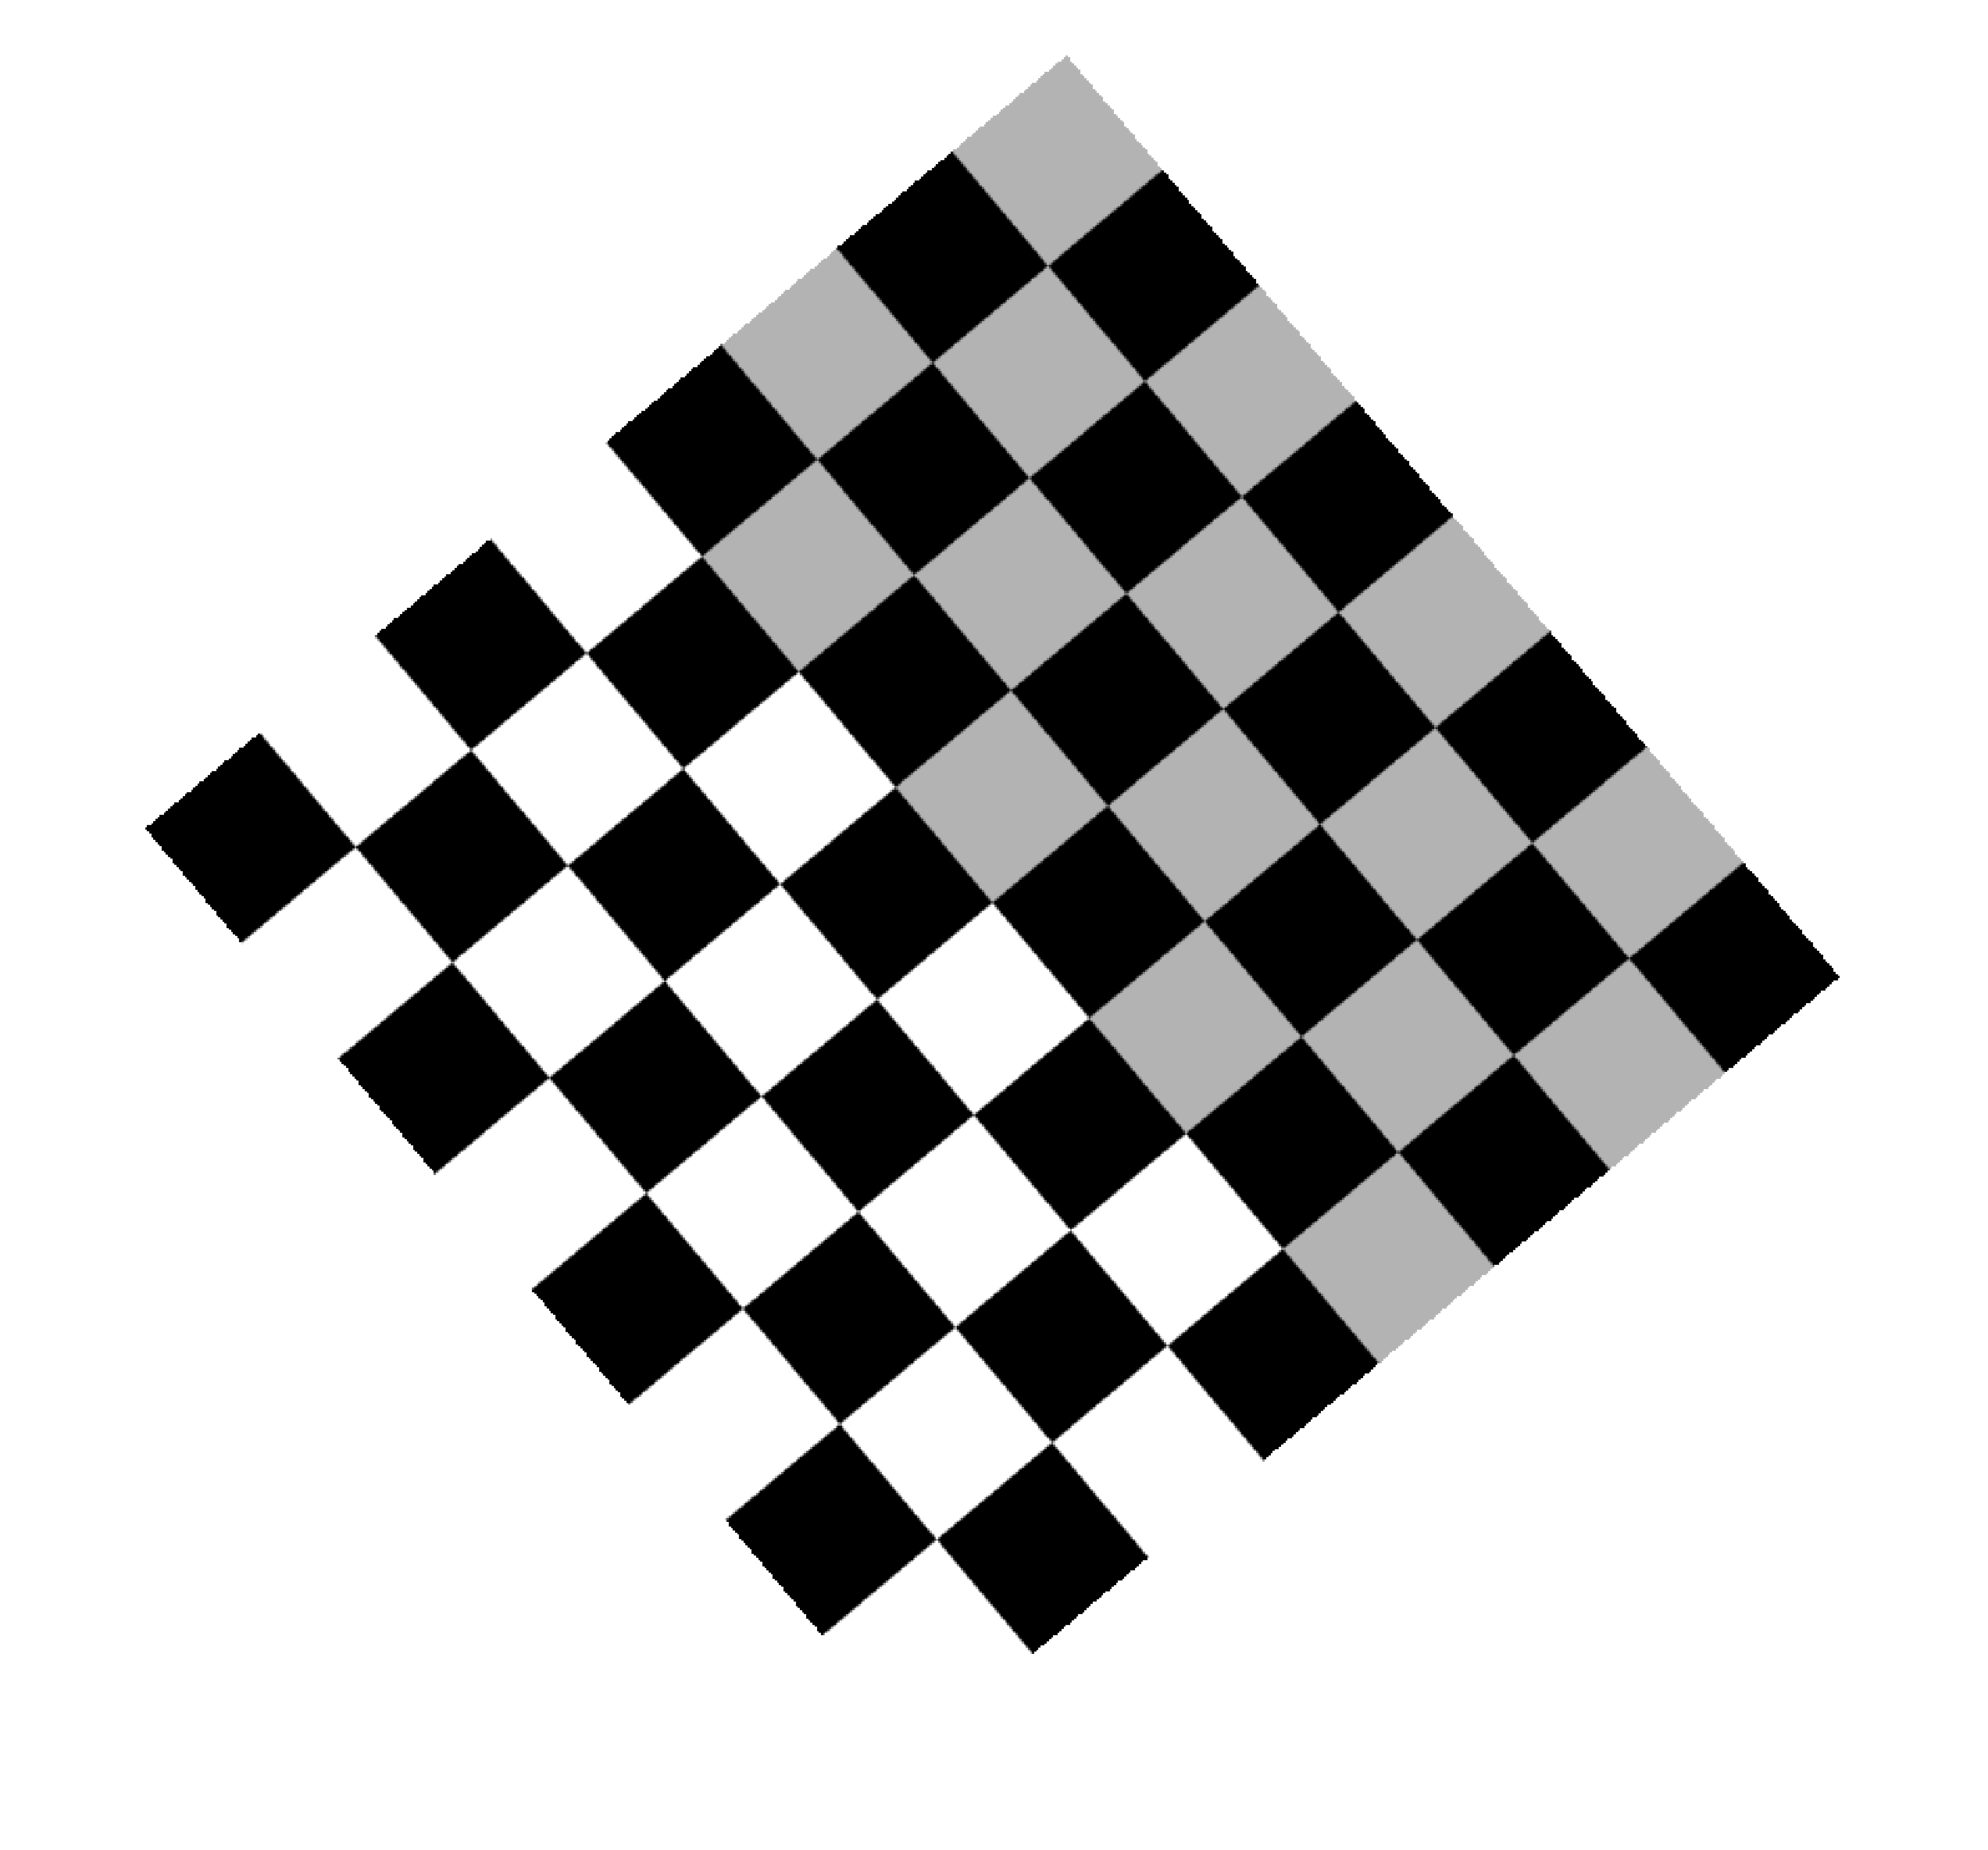
\includegraphics[height=.5\linewidth,width=.5\linewidth]{figures/registration/transforms/similarity.png}
				}
			}
			\)
		\end{tabular}
		\caption{Rigid transformation (isometry)} \label{fig:rigidtransformation}
	\end{subfigure}
	\begin{subfigure}{\linewidth}
		\centering
		\begin{tabular}{>{\centering}p{3cm}c}
			\(
			\begin{bmatrix}
				a & b & t_x \\
				c & d & t_y \\
				0 & 0 & 1   \\
			\end{bmatrix}
			\)
			 &
			\(
			\vcenter{
				\hbox{
					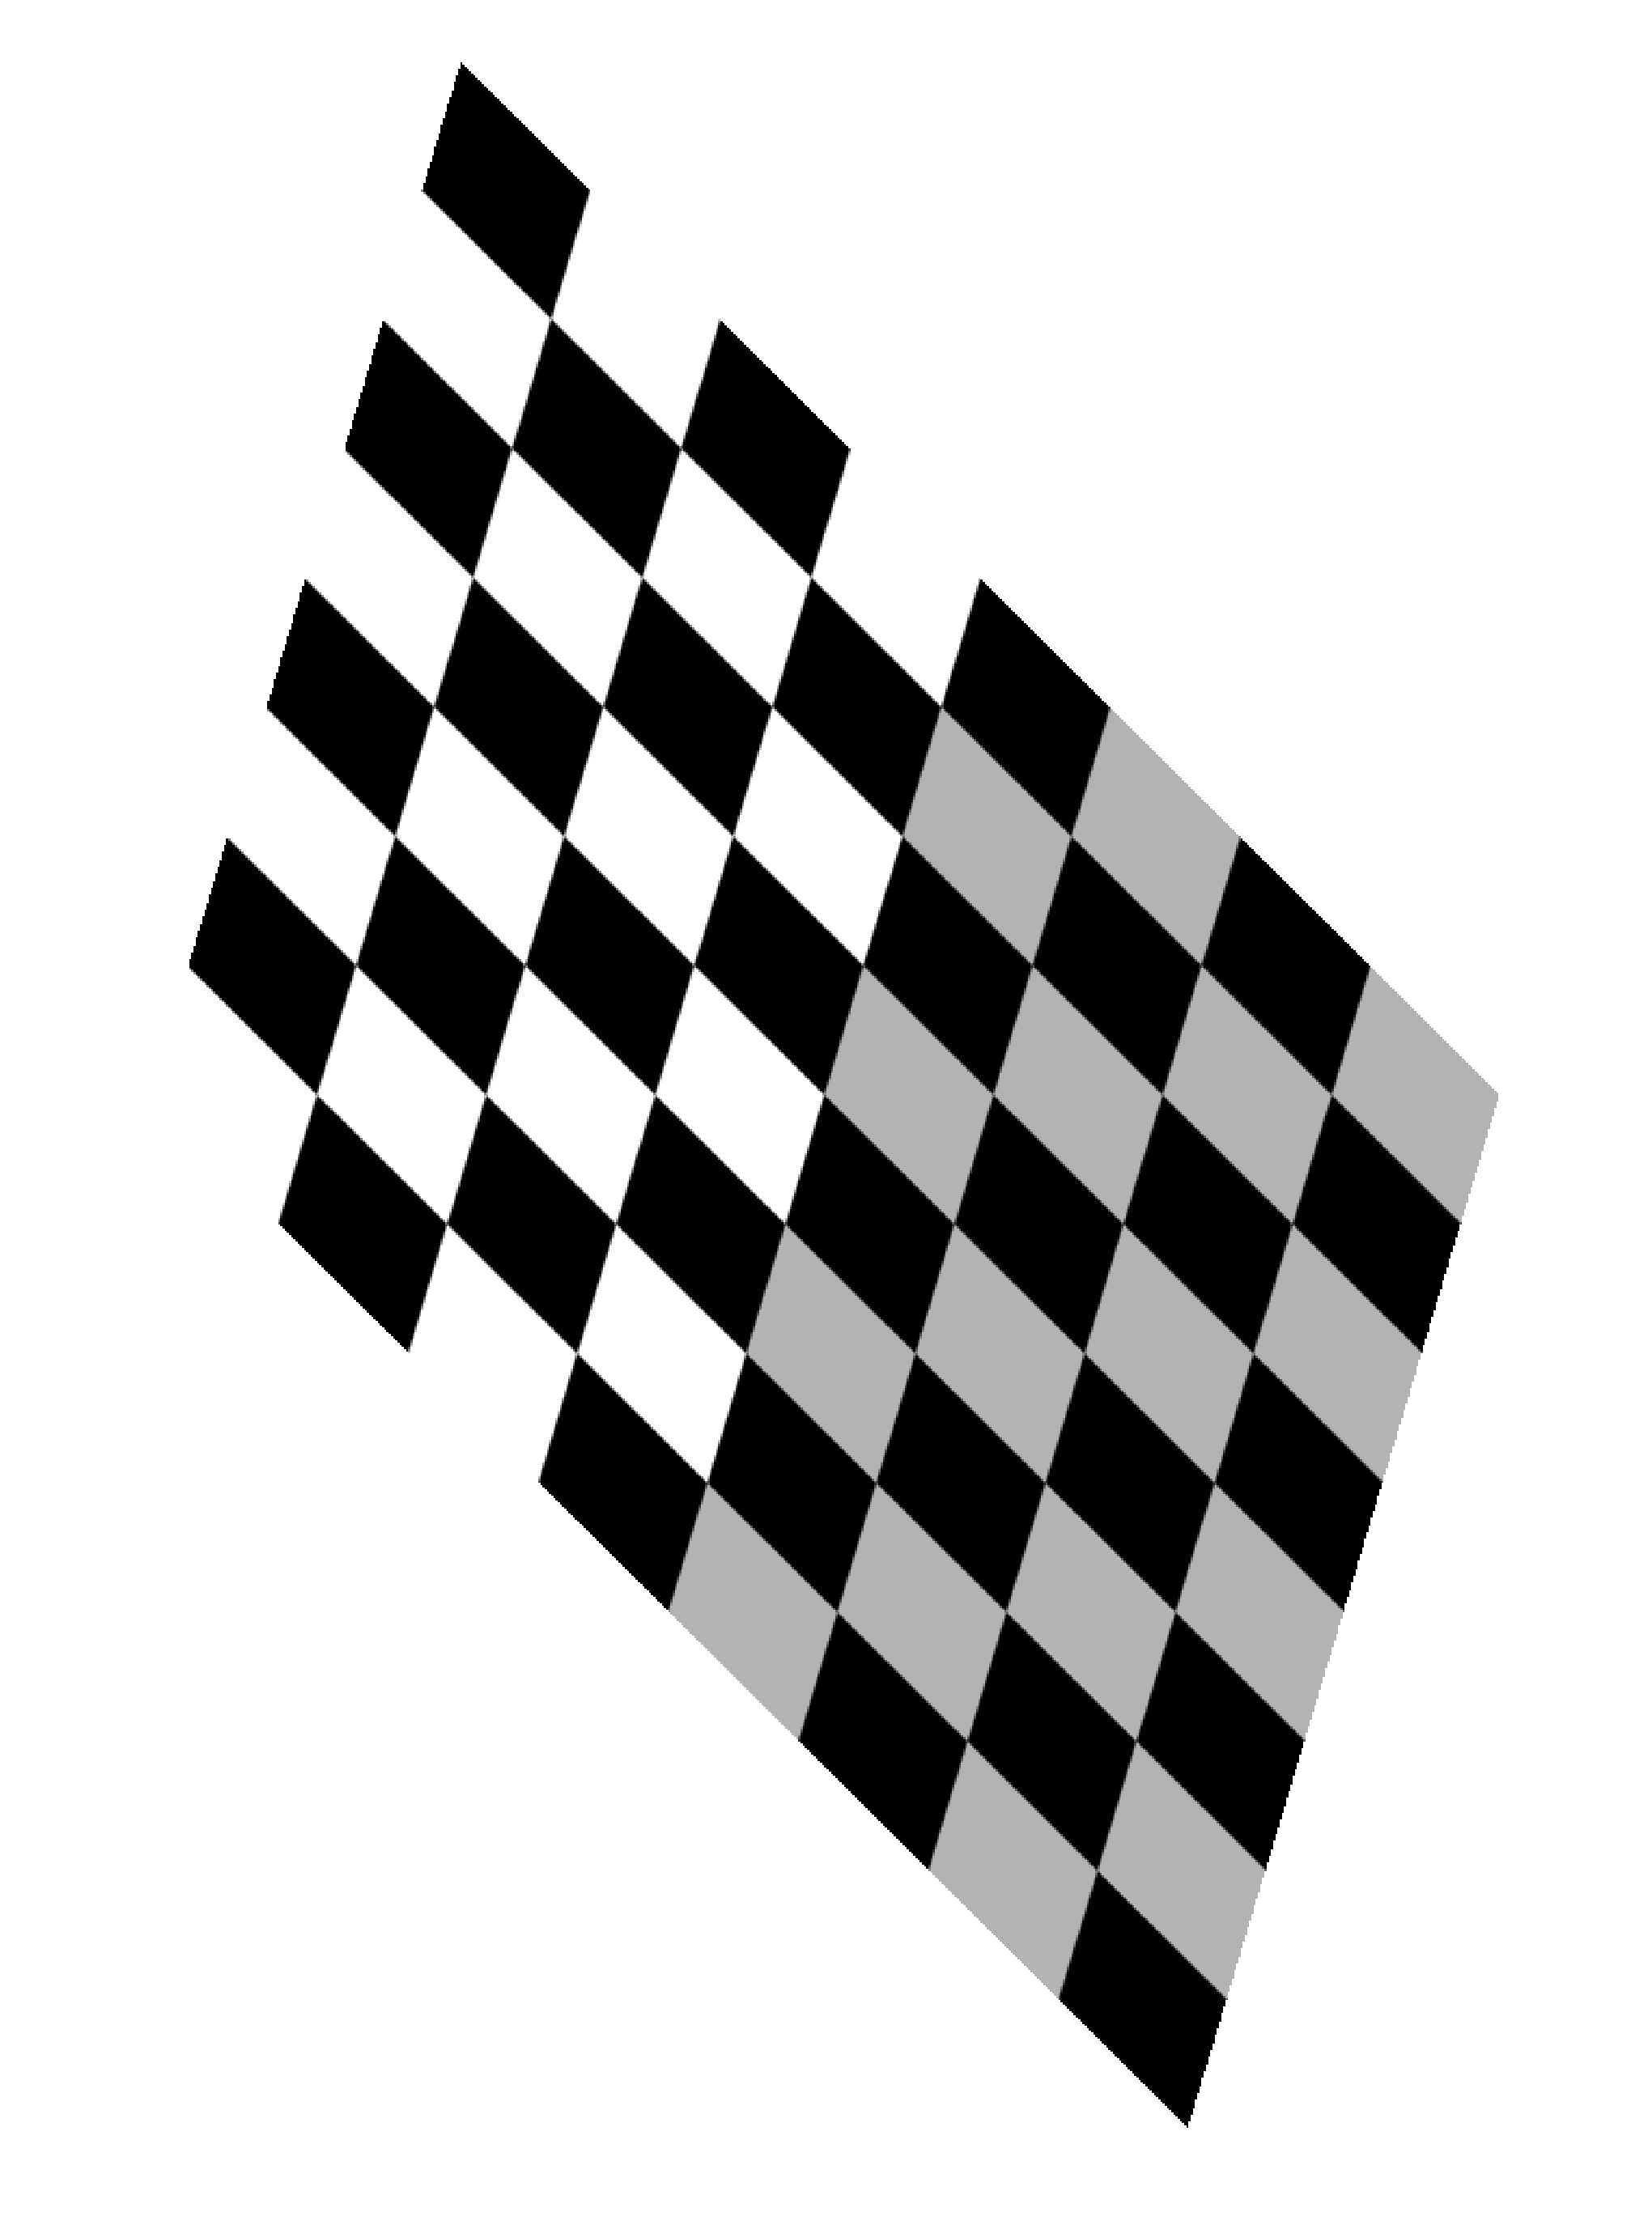
\includegraphics[height=.5\linewidth,width=.5\linewidth]{figures/registration/transforms/affine.png}
				}
			}
			\)
		\end{tabular}
		\caption{Affine transformation} \label{fig:affinetransformation}
	\end{subfigure}
	\begin{subfigure}{\linewidth}
		\centering
		\begin{tabular}{>{\centering}p{3cm}c}
			\(
			\begin{bmatrix}
				a & b & c \\
				d & e & f \\
				g & h & i \\
			\end{bmatrix}
			\)
			 &
			\(
			\vcenter{
				\hbox{
					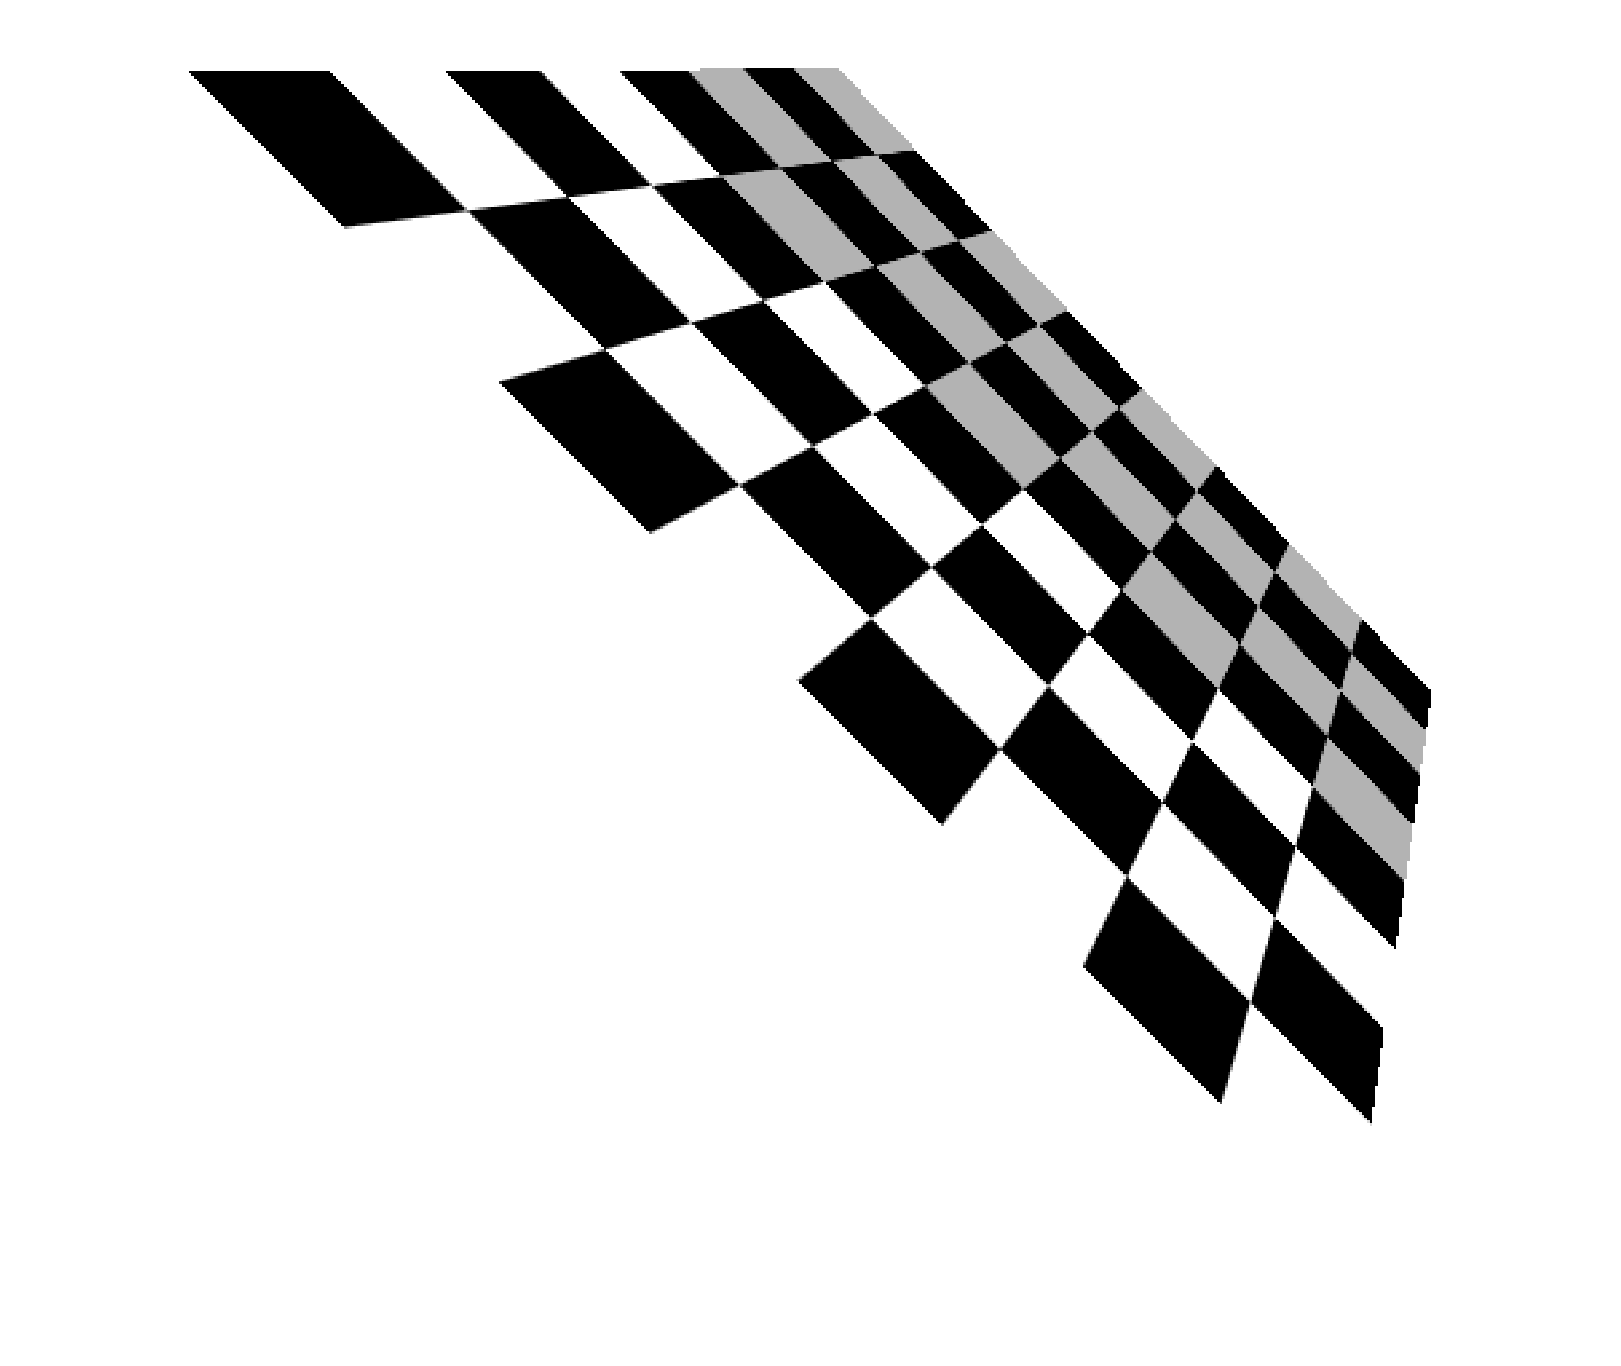
\includegraphics[height=.5\linewidth,width=.5\linewidth]{figures/registration/transforms/projective.png}
				}
			}
			\)
		\end{tabular}
		\caption{Projective (perspective) transformation (homography)} \label{fig:projectivetransformation}
	\end{subfigure}
	\begin{subfigure}{\linewidth}
		\centering
		\begin{tabular}{>{\centering}p{4cm}c}
			\(
			\begin{bmatrix}
				a(x,y) & b(x,y) & c(x,y) \\
				d(x,y) & e(x,y) & f(x,y) \\
				g(x,y) & h(x,y) & i(x,y) \\
			\end{bmatrix}
			\)
			 &
			\(
			\vcenter{
				\hbox{
					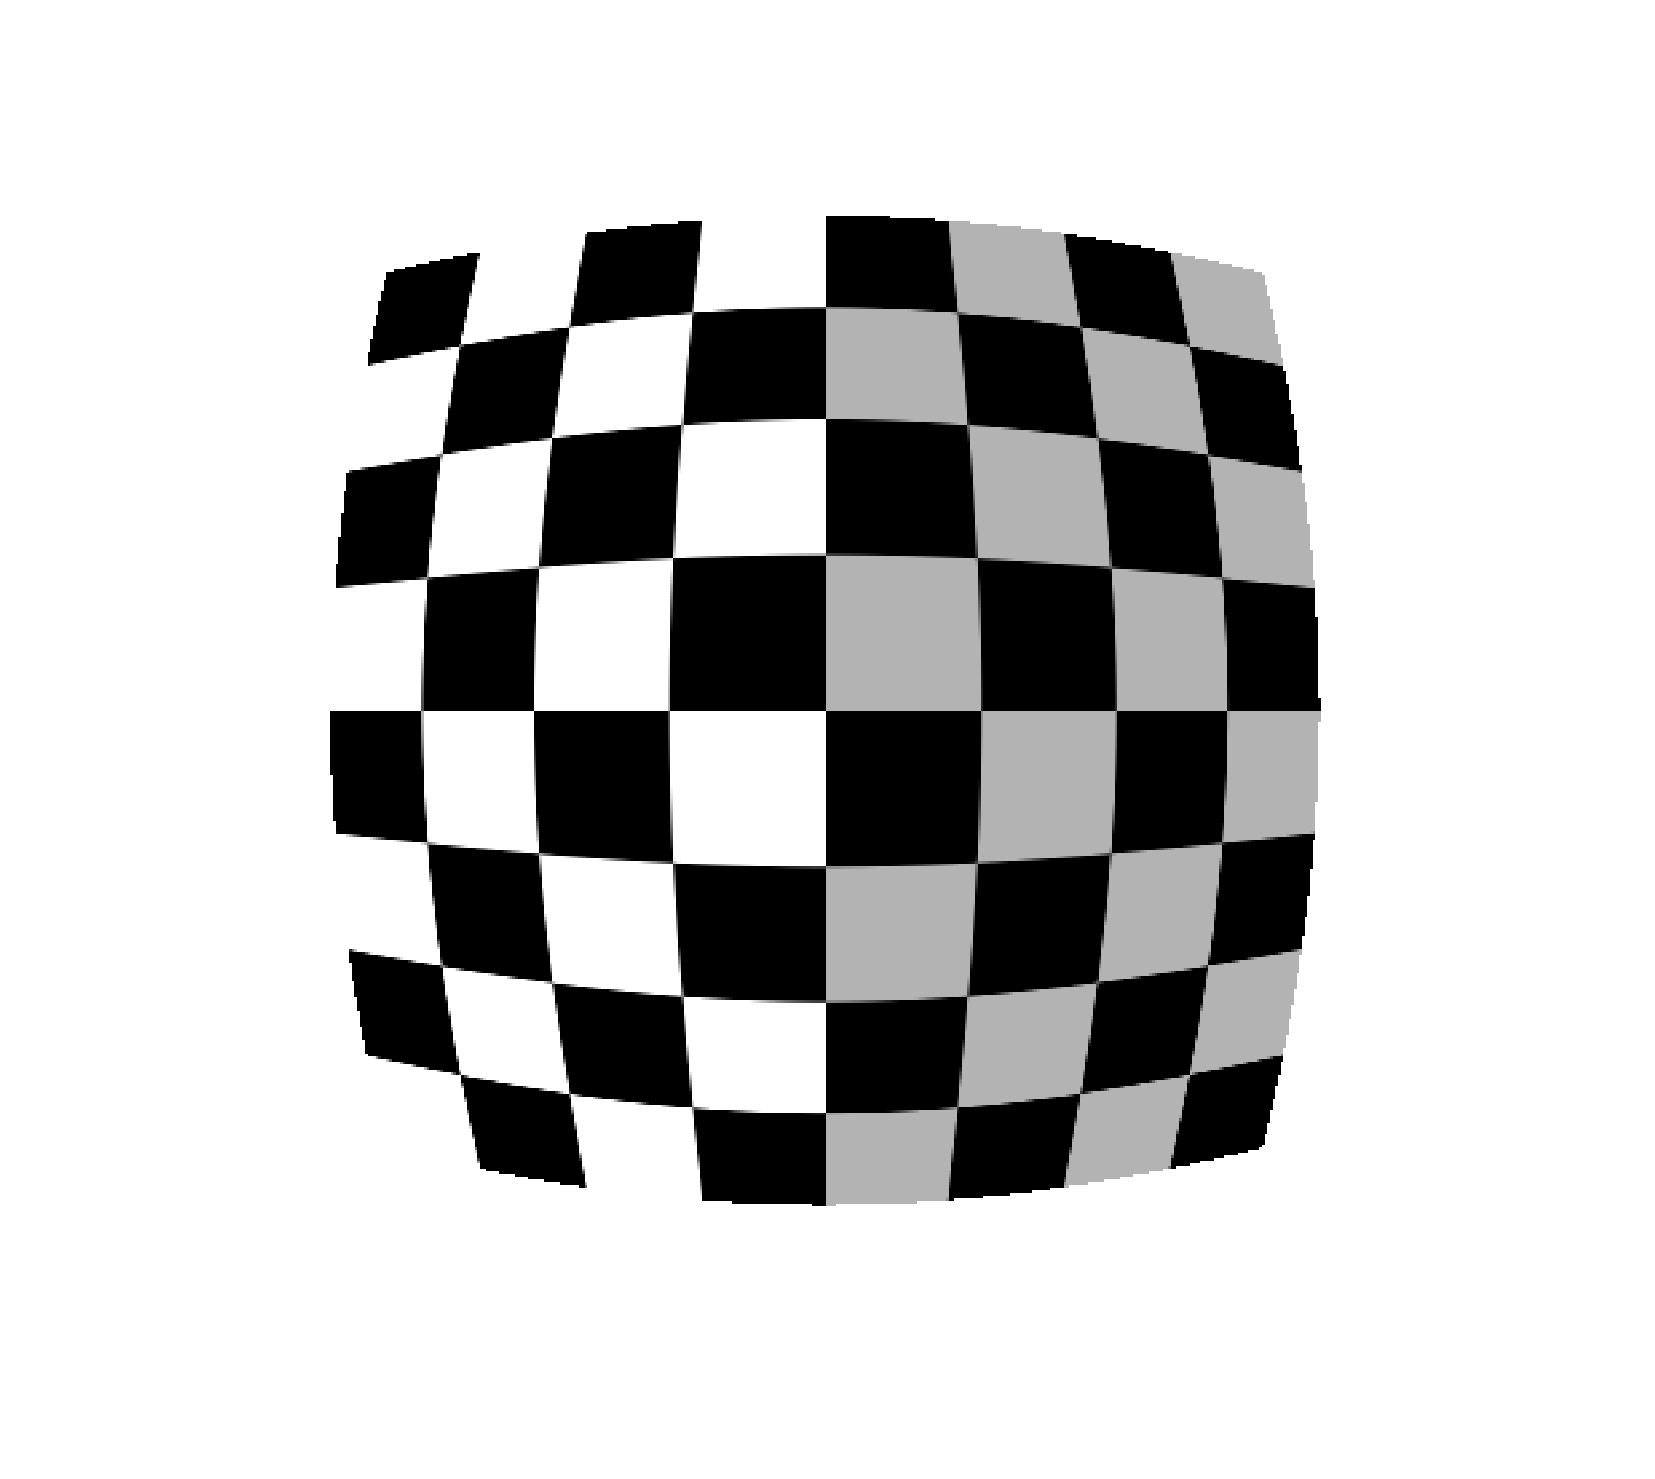
\includegraphics[height=.5\linewidth,width=.5\linewidth]{figures/registration/transforms/barrel.png}
				}
			}
			\)
		\end{tabular}
		\caption{Elastic transformation} \label{fig:elastictransformation}
	\end{subfigure}
	\caption[Compact Routing Example]{Different transformation classes (in homogeneous coordinates) along with realized examples.}
	\label{fig:transformations}
\end{figure}

After feature matching is sucessfully completed the transformation function \(f\) is constructed (see eqn.~\eqref{eqn:registration}).
%
This consists of choosing a transformation type (see figure~\ref{fig:transformations}) and estimating the parameters necessary to uniquely determine the transformation.
%
The transformation type is partially informed by knowledge of the geometry of the displacements (rigid, affine, projective) and partially informed by computational efficiency (more general transformation have more parameters).
%
There are broadly two perspectives on constructing the transformation \(f\): the global perspective which aims to model motion as a map of the image as a whole and the local perspective which aims to model motion as a deformation of individual pixels.
%
%These two perspectives naturally correspond to a globally (see figures~\ref{fig:rigidtransformation}, ~\ref{fig:affinetransformation}, ~\ref{fig:projectivetransformation}) or locally defined transformation \(f\) (see figure~\ref{fig:elastictransformation}).
%
We first quickly cover global algorithms and then move on to more powerful, and more interesting, local algorithms.

\subsubsection{Global Algorithms}

The most commonly used global model is the rigid transformation (see figures~\ref{fig:rigidtransformation}), which in homogeneous coordinates\anote{homogeneous} is defined:
\begin{equation}
	\begin{bmatrix}
		x' \\
		y' \\
		1  \\
	\end{bmatrix} =
	\begin{bmatrix}
		\cos(\theta) & -\sin(\theta) & t_x \\
		\sin(\theta) & \cos(\theta)  & t_y \\
		0            & 0             & 1   \\
	\end{bmatrix}
	\begin{bmatrix}
		x \\
		y \\
		1 \\
	\end{bmatrix}
	\label{eqn:rigidparams}
\end{equation}
The unknown parameters \((\theta, t_x, t_y)\) in eqn.~\eqref{eqn:rigidparams} can be estimated by expanding \(x', y'\) to using Taylor series
\begin{equation}
	\begin{split}
		x' &= t_x + x\left( 1 - \frac{\theta^2}{2} \right) - y\theta  + O(\theta^3) \\
		y' &= t_y + x \theta  + y\left( 1 - \frac{\theta^2}{2} \right) + O(\theta^3)
	\end{split}
	\label{eqn:rigidtaylor}
\end{equation}
Note that this is only valid for small angles \(\theta\) (the small-angle approximation\cite{keren1988}).
%
Truncating eqns.~\eqref{eqn:rigidtaylor} to first or second order and substituting data from matched features yields a system of linear equations.
%
Given that often there are many more matched features than unknowns in eqns.~\eqref{eqn:rigidtaylor} such a system is overdetermined; a unique solution can be determined using regularized least-squares.
%
In order to make this process more efficient and increase accuracy Keren \etal\cite{keren1988} use a Gaussian pyramid (see figure~\ref{fig:siftpyramid} and corresponding discussion in section~\ref{sec:sift}) to iteratively refine estimates at higher and higher resolutions.
%
In the more general case of a projective transformation (a perspective shift) the transformed pixel coordinates are
\begin{equation}
	\begin{split}
		x' & = \frac{ax+by+c}{gx+hy+i} \\
		y' & = \frac{dx+ey+f}{gx+hy+i}
		\label{eqn:projectivetf}
	\end{split}
\end{equation}
and similarly the unknowns (\(a,b,\dots\), etc.) can be estimated from matched feature correspondence data.

\subsubsection{Local Algorithms}
\paragraph{Splines}
\paragraph{Optical Flow}
\begin{figure}[!htbp]
	\begin{subfigure}{\linewidth}
		\centering
		\begin{adjustbox}{height=.7\textwidth}
			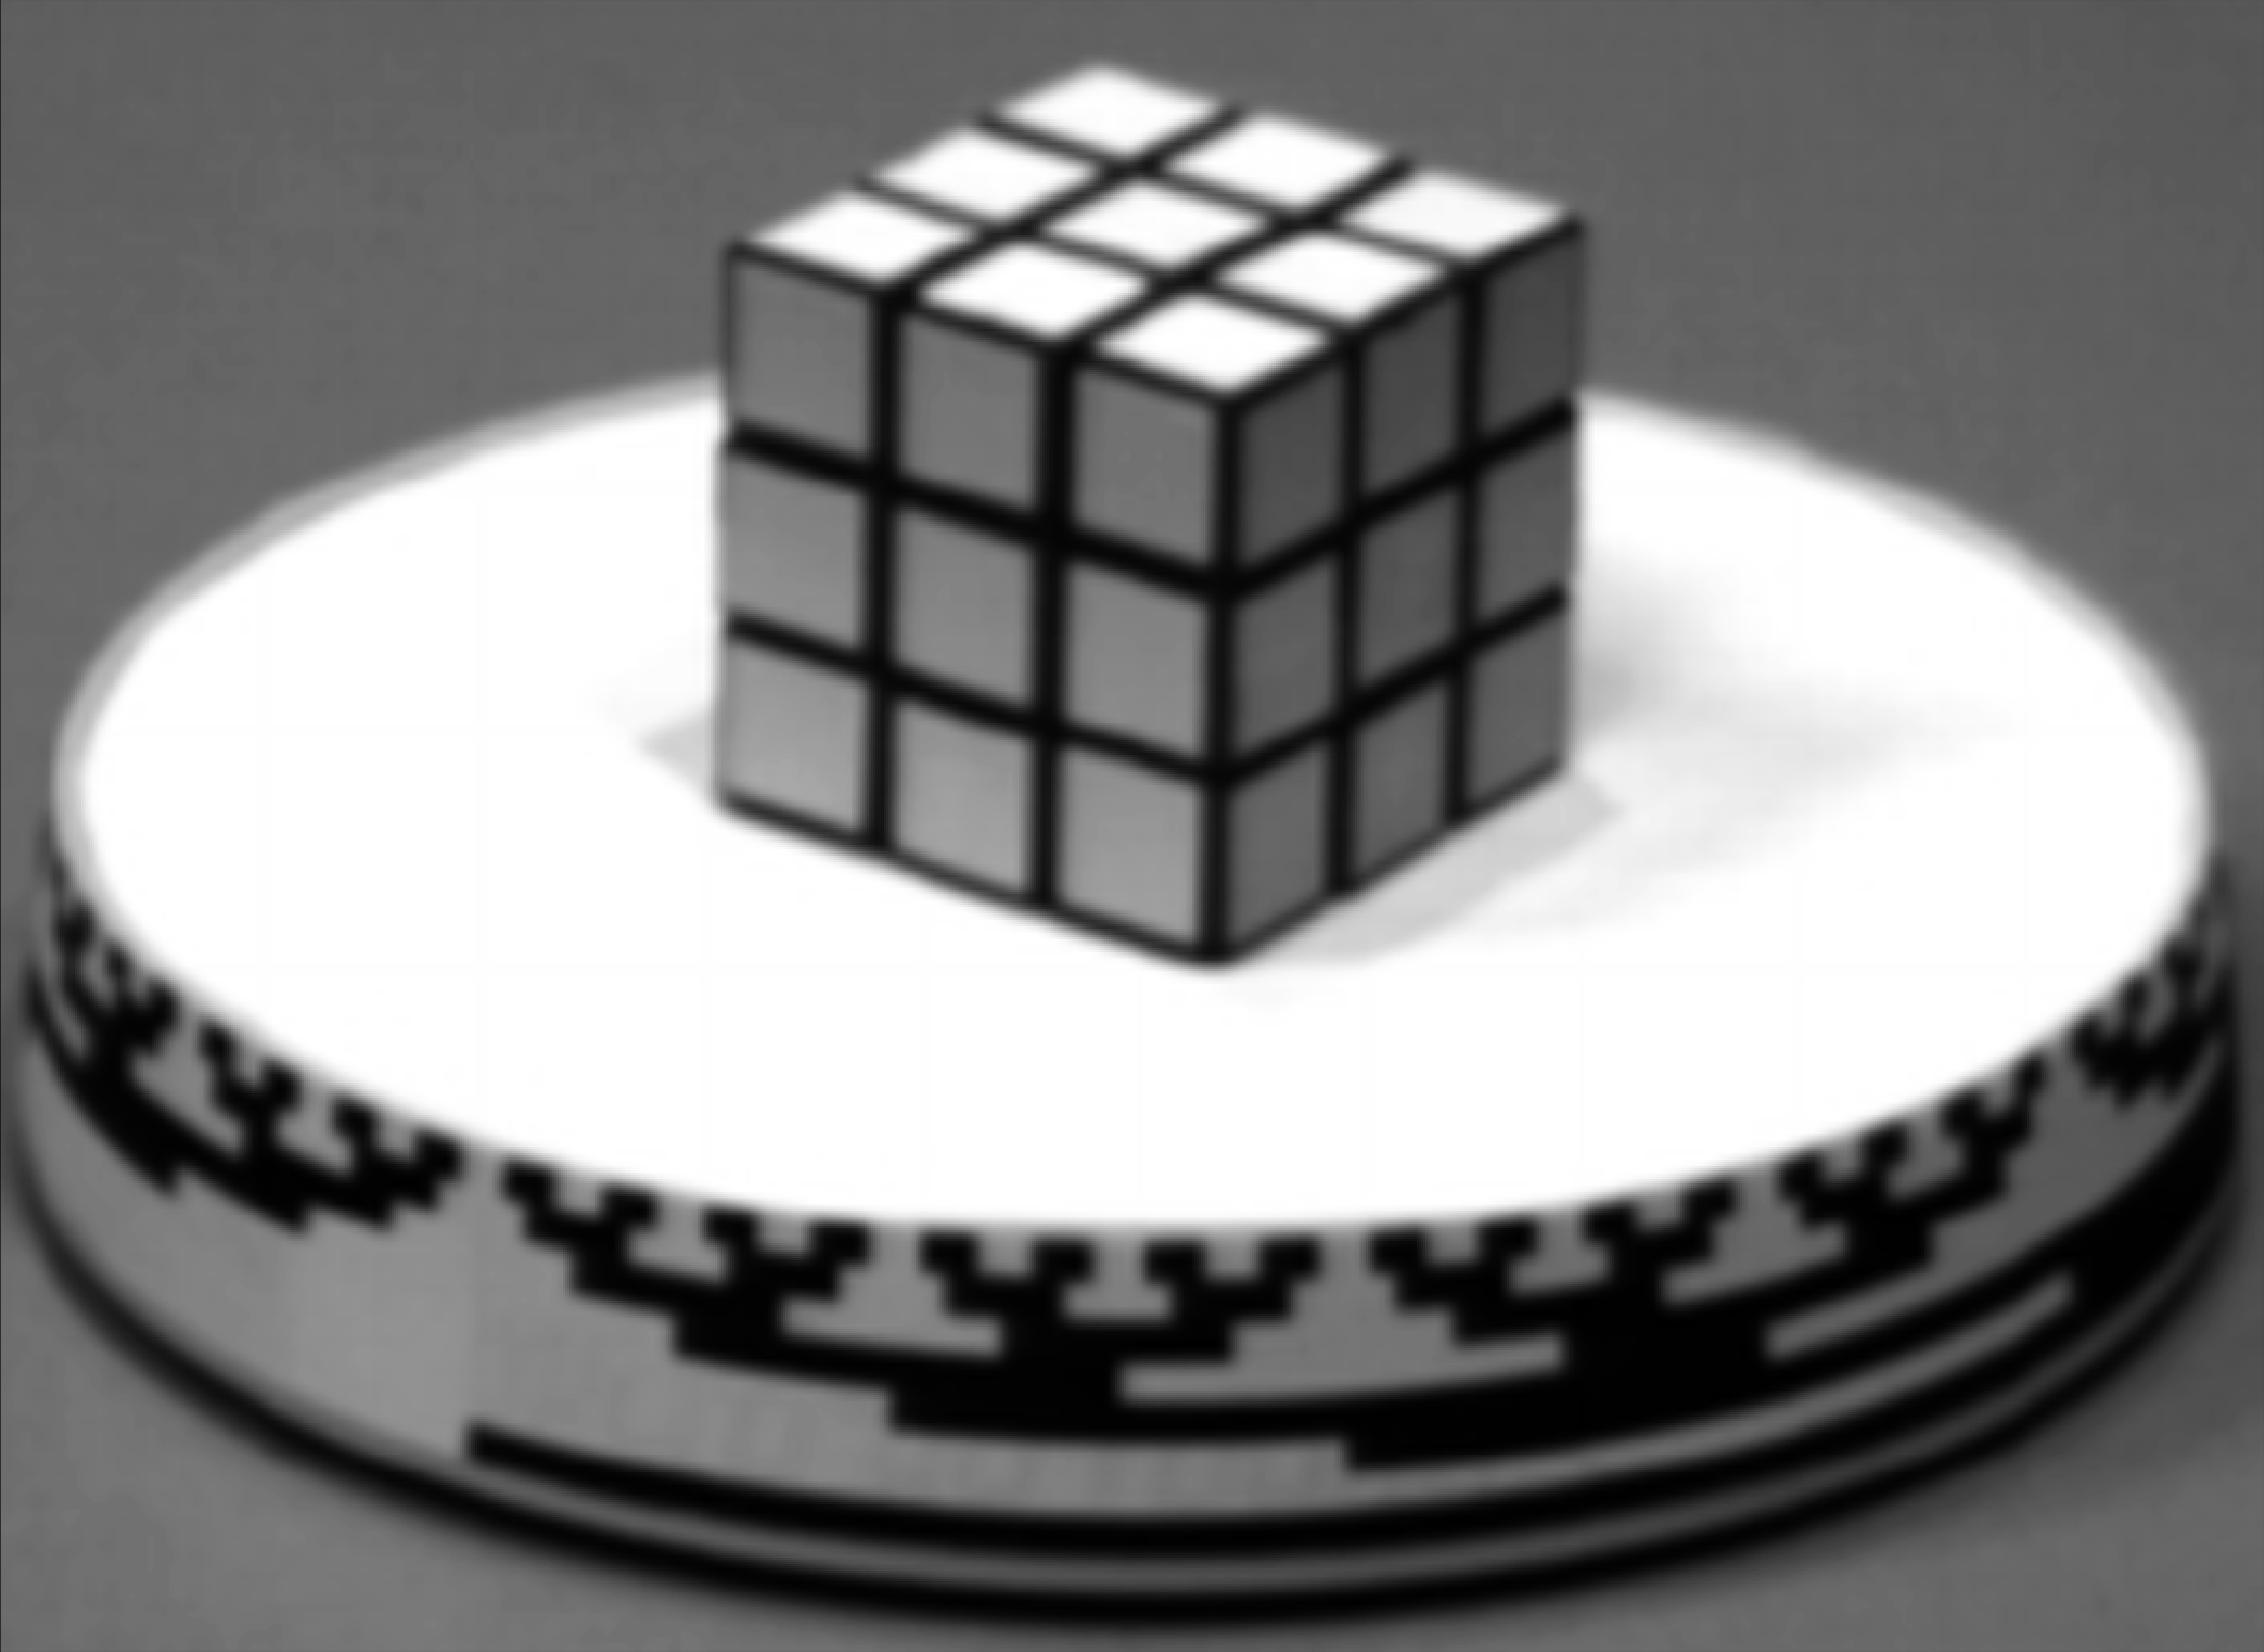
\includegraphics[]
			{figures/registration/optical_flow/reference_image.png}
		\end{adjustbox}
		\caption{Reference image.} \label{fig:refoptical}
	\end{subfigure}
	\vskip\baselineskip
	\begin{subfigure}{\linewidth}
		\centering
		\begin{adjustbox}{height=.7\textwidth}
			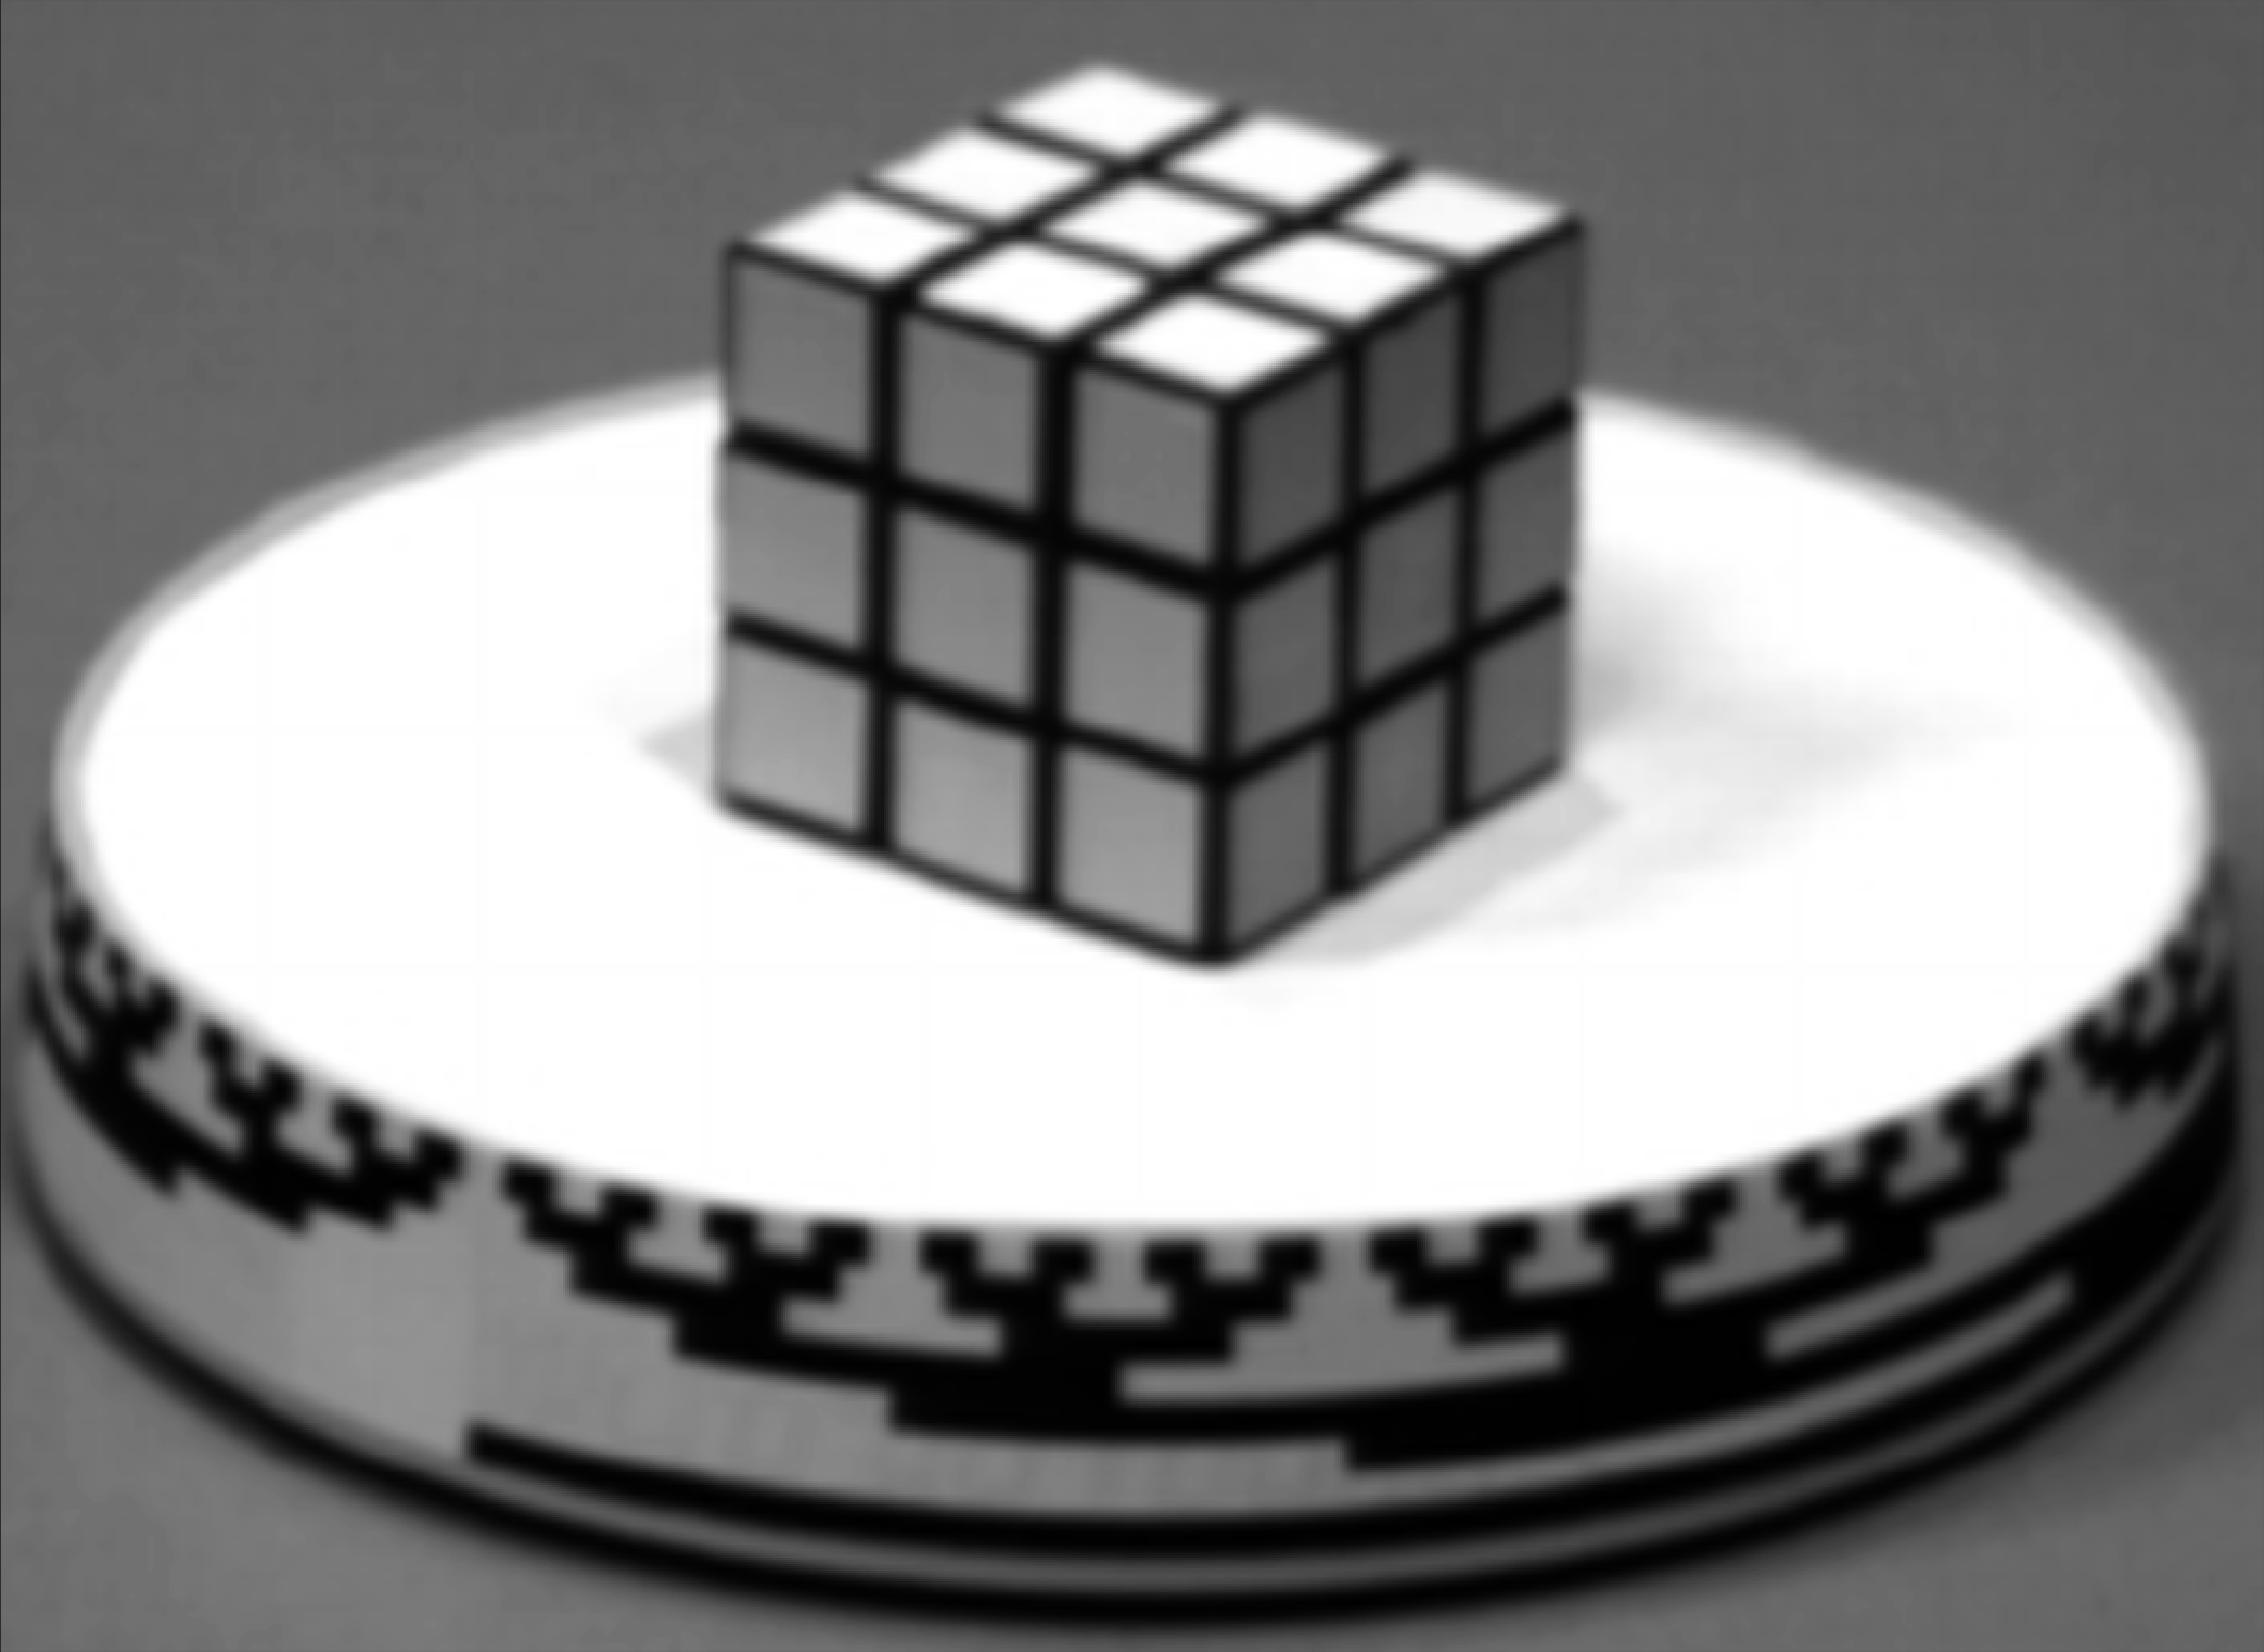
\includegraphics[]
			{figures/registration/optical_flow/moving_image.png}
		\end{adjustbox}
		\caption{Moving/displaced image.} \label{fig:movoptical}
	\end{subfigure}
	\vskip\baselineskip
	\begin{subfigure}{\linewidth}
		\centering
		\begin{adjustbox}{height=.7\textwidth}
			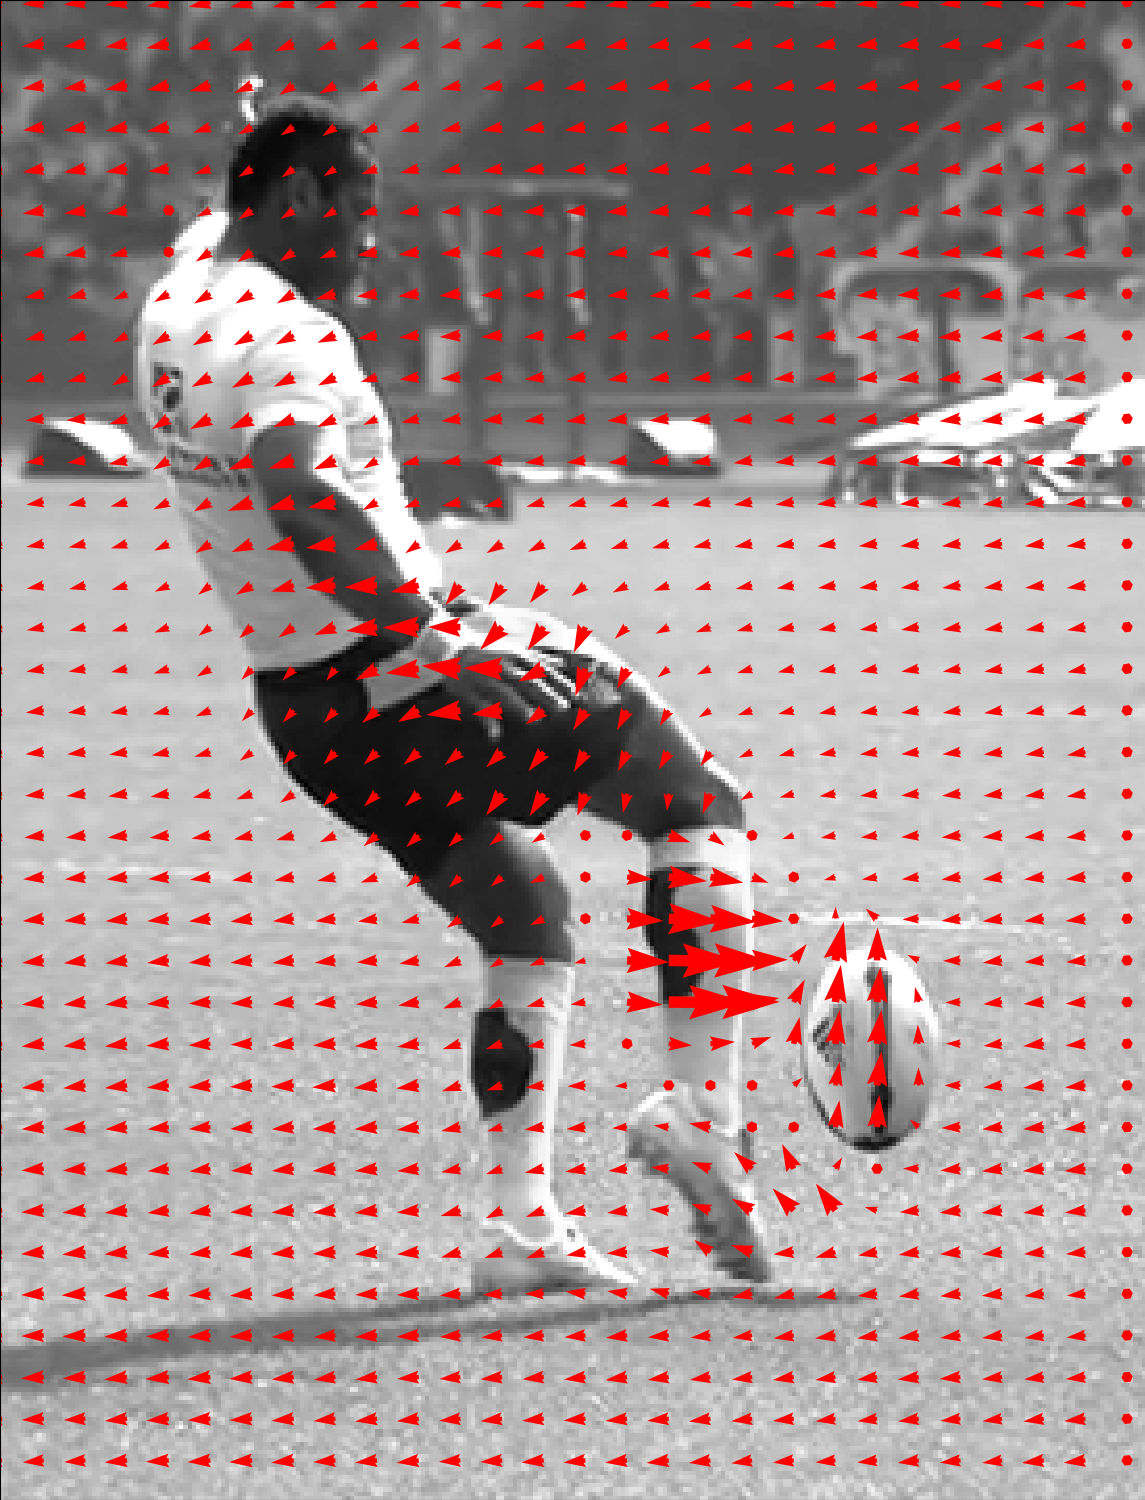
\includegraphics[]
			{figures/registration/optical_flow/flow.png}
		\end{adjustbox}
		\caption{Velocity field.} \label{fig:fieldoptical}
	\end{subfigure}
	\caption{Optical flow.}\label{fig:opticalflow}
\end{figure}

The most general and most interesting framing of the problem of local transformation is \textit{optical flow}.
%
Optical flow is the apparent motion of objects, surfaces, and edges in a scene caused by the relative motion between an observer and a scene.
%
It is most often represented as a velocity field over the individual point sources in the scene (see figure~\ref{fig:opticalflow}).
%
This velocity field can be used to define a mapping between pixels in the displaced image and the reference image (in a sense propagating the pixels backwards in time).

One approach to computing optical flow is based on treating pixel intensity as a \textit{conserved quantity}.
%
Let \(X(x,y,t)\) be pixel intensity over a sequence of images (i.e., the images per se).
%

\noindent Then define
\begin{equation*}
	Q(t) \coloneqq \iint_R X(x,y,t) \dif R
\end{equation*}
be the total pixel intensity over some image region \(R\), and assume \(Q\) is differentiable in \(t\) (we deal with discretization in the forthcoming).
%
\(Q\) obeys a \textit{continuity equation}:
\begin{equation}
	\od{}{t} Q(t) + \oint_{\partial R} \mathbf{j} \cdot \mathbf{n}\, \dif l = \Sigma
	\label{eqn:intcontinuity}
\end{equation}
where \(\partial R\) is the closed boundary of \(R\) (\(\dif l\) is the differential line element of \(\partial R\)), \(\mathbf{n}\) is unit length and normal to \(\partial R\), \(\mathbf{j}\) is the intensity flux (i.e., rate of flow of the intensity) through \(\partial R\), and \(\Sigma\) is the sum of all intensity sources and intensity sinks in \(R\).
%
Equation~\eqref{eqn:intcontinuity} expresses the fact that the change in total pixel intensity in the region \(R\) over time is equal to net intensity creation minus net flux through the boundary of the region.
%
By the Stokes' theorem\anote{stokes} and interchanging the order of integration and differentiation
%\begin{align}
%	\od{}{t} Q(t) + \oint_{\partial R} \mathbf{j} \cdot \mathbf{n}\, \dif l &=  \\
%	\od{}{t} \iint_R X(x,y,t) \dif R + \iint_R \nabla \cdot \mathbf{j}\, \dif R &= \\
%	 \iint_R \pd{X}{t} \dif R + \iint_R \nabla \cdot \mathbf{j}\, \dif R &= \\
%	\iint_R \pd{X}{t} + \nabla \cdot \mathbf{j}\,  \dif R &= \Sigma
%\end{align}
\begin{align*}
	\od{}{t} Q(t) + \oint_{\partial R} \mathbf{j} \cdot \mathbf{n}\, \dif l & = \od{}{t} \iint_R X(x,y,t) \dif R + \iint_R \nabla \cdot \mathbf{j}\, \dif R \\
	& = \iint_R \pd{X}{t} \dif R + \iint_R \nabla \cdot \mathbf{j}\, \dif R         \\
	& = \iint_R \left[ \pd{X}{t} + \nabla \cdot \mathbf{j} \right]  \dif R = \Sigma
\end{align*}
Then the corresponding differential form for eqn.~\eqref{eqn:intcontinuity} is
\begin{equation}
	\pd{X}{t} + \nabla \cdot \mathbf{j} = \sigma
	\label{eqn:diffcontinuity}
\end{equation}
where now \(\sigma\) is net intensity creation per unit area.
%
This is a generalized advection equation\anote{advection}.
%
If pixel intensity is a conserved quantity (i.e., no net creation) eqn.~\eqref{eqn:diffcontinuity} becomes
\begin{equation}
	\pd{X}{t} + \nabla \cdot \mathbf{j} = 0
	\label{eqn:conservintent}
\end{equation}
By definition \(\mathbf{j} = X\mathbf{u}\) where \(\mathbf{u} \coloneqq (u_1(x,y), u_2(x,y))\) is the velocity field (over all the points in the image).
%
If we further assume that the intensity flow is incompressible (i.e., intensity density remains constant as it is advected by the point sources) then \(\nabla \cdot \mathbf{u} = 0\) and eqn~\eqref{eqn:conservintent} becomes
\begin{equation}
	\pd{X}{t} + \mathbf{u} \cdot \nabla X = 0
	\label{eqn:intensityconstr}
\end{equation}

Equation~\eqref{eqn:intensityconstr} is called the \textit{optical flow constraint equation}\cite{perez2013tv}.
%
Note that the constraint equation is a single linear equation in two unknowns (the components of \(\mathbf{u}\)) and is therefore under-determined.
%
\begin{figure*}
    \tikzset{
        aperture/.pic={
                \pgfmathsetmacro\cs{sqrt(1.5*cos(#1-45)^2/2)};
                \path [draw=black, rotate=#1, pattern=north east lines]
                    (-6/4,-6/2) rectangle (6/4,6/2);
                \path [fill=white, draw=black, even odd rule]
                    circle [radius=4/3] (-2,-2) rectangle (2,2);

                \draw[bluearrow, rotate=#1, line width=0.5mm] (0,0) -- node [above] {\small{\(\mathbf{u}\)}} (0,1.5);
                \draw[redarrow, line width=0.5mm] (0,0) -- node [above] {\small{\(\nabla X\)}} (-1.5,1.5);
                \draw[greenarrow, line width=0.5mm] (0,0) -- node [left] {\small{\(\nabla X \cdot \mathbf{u}\)}} (-\cs,\cs);
            }
    }
    \centering
    \begin{subfigure}[b]{0.3\textwidth}
        \centering
        \begin{adjustbox}{height=\textwidth}
            \begin{tikzpicture}
                \pic {aperture={45}};
            \end{tikzpicture}
        \end{adjustbox}
        \caption{Diagonal motion. \(\nabla X \cdot \mathbf{u}\) is maximum and therefore optical flow directly corresponds to motion.}
        \label{fig:diagbarber}
    \end{subfigure}
    \hfill
    \begin{subfigure}[b]{0.3\textwidth}
        \centering
        \begin{adjustbox}{height=\textwidth}
            \begin{tikzpicture}
                \pic {aperture={0}};
            \end{tikzpicture}
        \end{adjustbox}
        \caption{Vertical motion. \(\nabla X \cdot \mathbf{u}\) is less than maximum and therefore optical flow fails to capture all of the motion.}
        \label{fig:vertbarber}
    \end{subfigure}
    \hfill
    \begin{subfigure}[b]{0.3\textwidth}
        \centering
        \raisebox{22pt}{
            \begin{adjustbox}{width=\textwidth}
                \begin{tikzpicture}
                    \pic {aperture={90}};
                \end{tikzpicture}
            \end{adjustbox}
        }
        \caption{Horizontal motion. \(\nabla X \cdot \mathbf{u}\) is less than maximum and therefore optical flow fails to capture all of the motion.}
        \label{fig:horizbarber}
    \end{subfigure}
    \caption{Barber-poll illusion. Each of the three motion measure as vertical optical flow.}
    \label{fig:barberpoll}
\end{figure*}
%
This is called the \textit{aperture problem} or the Barber-poll illusion (see figure~\ref{fig:barberpoll}) because any motion perpendicular to image gradients \(\nabla X\) (i.e., edges) isn't captured by the constraint: to wit if 
\[\mathbf{u}' \cdot \nabla X= 0\] 
then 
\[
	\pd{X}{t} + \left(\mathbf{u} + \mathbf{u}' \right) \cdot \nabla X = \pd{X}{t} + \mathbf{u} \cdot \nabla X = 0
\]
%
Therefore additional constraints need to be imposed in order to uniquely determine \(\mathbf{u}\).
%
The first such additional constraint was the \textit{spatial coherence constraint} proposed by Lucas\etal~\cite{lucas1981iterative}: assume a pixel's neighbors have the same velocity \(\mathbf{u}\).
%
For example using a \(5 \times 5\) window around a given pixel yields a \(5\times5 = 25\) equation over-determined system (solved using least-squares).

Regularizers can also be used to resolve the aperture problem. 
%
Defining \(\rho(\mathbf{u})\) as the left-hand side of eqn.~\eqref{eqn:intensityconstr}, Horn \etal~\cite{horn1993determining} propose the functional
\begin{multline}
	E(\mathbf{u}) \coloneqq
	\int_R \left[ |\rho(\mathbf{u})|^2 + \alpha \left( | \nabla u_1 |^2 + | \nabla u_2 |^2\right) \right] \dif R
	\label{eqn:linearhorn}
\end{multline}
where \(| \nabla u_1 |^2\) is the \(L_2\) norm of \(\nabla u_1 = (\pd{u_1}{x}, \pd{u_1}{y})\).
%
\(E(\mathbf{u})\) acts a smoothing regularizer, constraining the acceleration of the flow (recall that \(\mathbf{u}\) is the velocity of the flow).
%
Note that \(\nabla u_1\) is not the first component of \(\nabla \cdot \mathbf{u} = (\pd{u_1}{x}, \pd{u_2}{y})\) and therefore not identitically zero (despite the assumption that  \(\nabla \cdot \mathbf{u} = 0\)).

Although eqn.~\eqref{eqn:intensityconstr}, along with Horn smoother, is an effective resolution to the problem of computing optical flows in continuous time it is unsuitable for images sampled discretely in time.
%
In such cases eqn.~\eqref{eqn:intensityconstr} is replaced by \( X_k(\bx + \mathbf{u}) - X_1(\bx)\), where \(\bx = (x,y)\), and then linearized around an initial velocity \(\mathbf{u}_1\):
\begin{multline}
	\nabla X_k (\bx + \mathbf{u}_1)\cdot (\mathbf{u} - \mathbf{u}_1)\, + \\ X_k(\bx + \mathbf{u}_1)  -  X_1(\bx) = 0
	\label{eqn:nonlinearconstr}
\end{multline}
Defining \(\rho'(\mathbf{u})\) as the left-hand side of eqn.~\eqref{eqn:nonlinearconstr}, the Horn smoother suitably adjusted is
\begin{equation}
	E'(\mathbf{u}) \coloneqq \int_R \left[ | u_1 |^2 + | u_2 |^2 + \lambda | \rho'(\mathbf{u}) |_1 \right] \dif R
	\label{eqn:nonlinearhorn}
\end{equation}
%
Perez \etal~\cite{perez2013tv} further relax this to a convex loss:
\begin{multline}
	E_{\theta}(\mathbf{u}, \mathbf{v}) \coloneqq \\
	\int_R \left[ | u_1 |^2 + | u_2 |^2 + \frac{1}{2\theta}| \mathbf{u} - \mathbf{v} |^2 + \lambda | \rho'(\mathbf{v}) |_1 \right] \dif R
	\label{eqn:relaxhorn}
\end{multline}
in order that they can alternate fixing one of \(\mathbf{u}, \mathbf{v}\) and minimizing with respect to the other.
%
Note that fixing \(\theta\) in eqn.~\eqref{eqn:relaxhorn} to be small pushes \(E_{\theta}(\mathbf{u}, \mathbf{v})\) to be small when \(\mathbf{u}\approx \mathbf{v}\) and therefore effectively minimizing eqn.~\eqref{eqn:nonlinearhorn}.